% ============================================================================
% IBFV: Iris-Boosted Fuzzy Vault for Multimodal Biometric Template Protection
% IEEE Conference/Transactions Format
% ============================================================================
\documentclass[conference]{IEEEtran}

% --- Packages ---
\usepackage{cite}
\usepackage{amsmath,amssymb,amsfonts}
\usepackage{amsthm}

\newtheorem{definition}{Definition}
\newtheorem{theorem}{Theorem}
\newtheorem{corollary}{Corollary}
\newtheorem{proposition}{Proposition}
\usepackage{algorithmic}
\usepackage{algorithm}
\usepackage{graphicx}
\usepackage{textcomp}
\usepackage{xcolor}
\usepackage{booktabs}
\usepackage{multirow}
\usepackage{array}
\usepackage{subcaption}
\usepackage{hyperref}
\usepackage{balance}
\usepackage{pifont}

% --- Custom commands ---
\newcommand{\IBFV}{\textsf{IBFV}}
\newcommand{\EER}{\mathrm{EER}}
\newcommand{\GAR}{\mathrm{GAR}}
\newcommand{\FAR}{\mathrm{FAR}}
\newcommand{\FRR}{\mathrm{FRR}}
\newcommand{\FHD}{\mathrm{FHD}}
\newcommand{\GFp}{\mathrm{GF}(p)}
\newcommand{\ie}{\textit{i.e.}}
\newcommand{\eg}{\textit{e.g.}}

\def\BibTeX{{\rm B\kern-.05em{\sc i\kern-.025em b}\kern-.08em
    T\kern-.1667em\lower.7ex\hbox{E}\kern-.125emX}}

\begin{document}

% ============================================================================
% TITLE
% ============================================================================
\title{Iris-Boosted Fuzzy Vault: Zero-Penalty Multimodal Biometric Template Protection via Elliptic Curve Cryptography}

\author{
\IEEEauthorblockN{Nallaparaju V. Suryanarayana Raju}
\IEEEauthorblockA{Department of Computer Science and Engineering\\
National Institute of Technology, Warangal, India\\
\textit{nv24csm2s04@student.nitw.ac.in}}
\and
\IEEEauthorblockN{Mulagala Sandhya}
\IEEEauthorblockA{Department of Computer Science and Engineering\\
National Institute of Technology, Warangal, India\\
\textit{m.sandhya@nitw.ac.in}}
% Add additional authors as needed
}

\maketitle

% ============================================================================
% ABSTRACT
% ============================================================================
\begin{abstract}
Multimodal fuzzy vault schemes for biometric template protection face a fundamental limitation: incorporating a second modality typically \emph{gates} decoding, causing rejection when the auxiliary modality fails---even if the primary biometric alone would have succeeded. This AND-fusion penalty is inherent to all prior multimodal vault architectures.

We propose the \emph{Iris-Boosted Fuzzy Vault} (\IBFV{}), which eliminates this penalty by deriving deterministic \emph{bonus polynomial points} from a stabilized iris key and injecting them into the fingerprint vault. If iris recovery succeeds, the decoder receives $K$ guaranteed-genuine points that reduce the Lagrange interpolation search space; if it fails, the system falls back to unimodal decoding with \emph{provably zero performance loss}. We prove $\EER_{\IBFV} \leq \EER_{\text{Uni}}$ for all configurations (Theorem~1) and demonstrate ISO/IEC~24745 compliance via security analysis against Ratha~\textit{et~al.}'s eight-point threat model, with ECDLP-based irreversibility ($\sim\!2^{128}$ operations).

Experiments on four FVC databases with CASIA-Iris-Interval across 960+ configurations and two evaluation setups show up to 61.3\% relative EER reduction (0.93\% vs.\ 2.40\% on FVC2004~DB1) with zero violations of the monotonicity guarantee across all 144 Setup~2 configurations and negligible deviations ($\leq 0.07$ pp) on 31 easy-database Setup~1 configurations. Comparison against four alternative architectures---AND-fusion, polynomial blinding, dense chaff seeding, and AES vault encryption---confirms that all gated designs degrade performance, with tightly coupled variants yielding EER~$\geq$~19\%.
\end{abstract}

\begin{IEEEkeywords}
Biometric template protection, fuzzy vault, elliptic curve cryptography, multimodal biometrics, iris recognition, fingerprint, cancelable biometrics
\end{IEEEkeywords}

% ============================================================================
% I. INTRODUCTION
% ============================================================================
\section{Introduction}
\label{sec:introduction}

Biometric authentication systems are increasingly deployed in high-stakes applications including border control, financial services, and national identity programs~\cite{jain2004multibiometrics}. Unlike passwords or tokens, biometric traits such as fingerprints and iris patterns are inherently tied to the individual, providing strong non-repudiation and resistance to credential sharing. However, this very permanence creates a critical vulnerability: once a stored biometric template is compromised, the underlying trait cannot be changed, revoked, or re-issued. A single database breach can permanently compromise a user's biometric identity across all systems that rely on that modality. The ISO/IEC~24745 standard~\cite{iso24745} formalizes three mandatory requirements for biometric template protection (BTP) schemes---\emph{irreversibility} (the stored template must not be invertible to recover the original biometric), \emph{unlinkability} (templates of the same user in different applications must be statistically independent), and \emph{revocability} (a compromised template must be replaceable)---that any deployable BTP scheme must satisfy.

The fuzzy vault scheme~\cite{juels2002fuzzy} is among the most widely studied BTP primitives~\cite{rathgeb2011survey}. It binds a cryptographic secret to biometric data by encoding the secret as a polynomial and evaluating it at biometric-derived coordinates; the genuine evaluation points are then hidden among randomly generated chaff points. Recovery requires presenting a sufficiently similar biometric query to identify enough genuine points for Lagrange interpolation. The scheme has been applied to fingerprint minutiae~\cite{clancy2003secure,nandakumar2007fuzzy,uludag2005fuzzy}, iris codes~\cite{hao2006combining}, and multimodal biometrics~\cite{nandakumar2008multibiometric}.

Recent work by Maurya~\textit{et~al.}~\cite{maurya2025enhancing} advanced the fingerprint fuzzy vault by replacing the traditional $\text{GF}(2^{16})$ arithmetic with elliptic curve cryptography (ECC) over the Brainpool~P256r1 curve~\cite{rfc5639}. The resulting scheme achieves vault entropy exceeding 7.7~bits per coordinate (vs.\ $\sim\!16$~bits for $\text{GF}(2^{16})$), renders dictionary attacks computationally infeasible under the ECDLP assumption, and attains EER as low as 0.005\% on FVC2002~DB1. However, unimodal fingerprint systems remain fundamentally limited: they are vulnerable to spoof attacks targeting a single modality, and their accuracy degrades sharply on challenging data (e.g., EER rises to 5.0\% on FVC2002~DB3, which contains low-quality thermal sweep captures).

Multimodal biometric systems~\cite{ross2003information,jain2004multibiometrics} address these limitations by fusing information from multiple biometric sources, improving both recognition accuracy and spoof resistance. However, integrating multimodal fusion into template protection schemes is substantially harder than in conventional (unprotected) recognition, because the cryptographic binding must accommodate multiple heterogeneous feature representations while preserving the security properties of the underlying primitive. Several multimodal fuzzy vault architectures have been proposed~\cite{nandakumar2008multibiometric,moon2010multibiometric}, but they share a common structural flaw: the second modality \emph{gates} the decoding process. Under this AND-fusion model, failure in the auxiliary modality causes the system to reject a genuine user---even when the primary biometric alone would have succeeded. This \emph{gating penalty} is not merely an implementation artifact; it is a mathematical consequence of the AND-fusion structure, since the joint genuine acceptance rate satisfies $\GAR_{\text{AND}} = \GAR_{\text{FP}} \times \GAR_{\text{Iris}} \leq \GAR_{\text{FP}}$ whenever $\GAR_{\text{Iris}} < 1$. For practical iris subsystems where $\GAR_{\text{Iris}} \approx 62\%$, over a third of all genuine users are penalized.

We propose the \emph{Iris-Boosted Fuzzy Vault} (\IBFV{}), a fundamentally different multimodal architecture that resolves this trade-off. Our key insight is that the iris modality should \emph{add evidence} to the polynomial reconstruction problem rather than \emph{gate access} to it. Concretely:

\begin{enumerate}
    \item We stabilize the iris code using a repetition-code fuzzy commitment~\cite{hao2006combining} with bit-interleaved error correction over $N = 49{,}152$ iris code bits, extracting a deterministic binary key with majority-vote block decoding.
    \item We derive $K$ \emph{virtual x-coordinates} from the iris key hash via a SHA-256-based pseudorandom function (PRF), evaluate the secret polynomial at these coordinates, and inject the resulting points into the vault as additional genuine polynomial evaluation points.
    \item During verification, if iris key recovery succeeds, the decoder receives $K$ \emph{guaranteed-genuine} polynomial points in addition to whatever fingerprint minutiae matched, strictly reducing the combinatorial search space for Lagrange interpolation from $\binom{|\mathcal{X}_{\text{FP}}|}{k+1}$ to $\binom{|\mathcal{X}_{\text{FP}}|}{k+1-K}$.
    \item If iris recovery fails, the decoder falls back to fingerprint-only decoding---\emph{identical to the unimodal system}---incurring provably zero penalty.
\end{enumerate}

We prove that under this construction, the \IBFV{} acceptance probability satisfies $\Pr[\text{Accept}_{\IBFV}] \geq \Pr[\text{Accept}_{\text{Uni}}]$ for every biometric sample pair and every parameter configuration (Theorem~\ref{thm:zero_penalty}), and demonstrate empirically that the improvement is substantial on challenging databases. Our contributions are:

\begin{itemize}
    \item \textbf{Novel architecture}: A multimodal fuzzy vault with a \emph{provable zero-penalty guarantee} and graceful degradation---the first multimodal fuzzy vault architecture where the auxiliary modality is guaranteed to never degrade performance.
    \item \textbf{Formal security analysis}: Compliance with all three ISO/IEC~24745 requirements (irreversibility, unlinkability, revocability), analyzed against Ratha~\textit{et~al.}'s~\cite{ratha2001enhancing} eight-point threat model with quantified brute-force resistance bounds.
    \item \textbf{Custom iris pipeline}: A complete iris recognition system---segmentation, rubber-sheet normalization, Log-Gabor encoding with fragile-bit masking, and fractional Hamming distance matching---integrated into the ECC fuzzy vault framework via fuzzy commitment with bit interleaving.
    \item \textbf{Comprehensive evaluation}: Experiments across four fingerprint databases (FVC2002~DB1--DB3, FVC2004~DB1), two evaluation setups, and five multimodal architectures totaling over 960 parameter configurations, with ablation studies on all key hyperparameters.
\end{itemize}

The remainder of this paper is organized as follows. Section~\ref{sec:related} surveys related work on biometric template protection, fuzzy vaults, and multimodal fusion. Section~\ref{sec:preliminaries} reviews elliptic curve cryptography, the ECC-based fuzzy vault, and iris fuzzy commitment. Section~\ref{sec:proposed} presents the \IBFV{} architecture with formal analysis. Section~\ref{sec:security} provides a comprehensive security analysis against ISO/IEC~24745 requirements. Section~\ref{sec:experiments} reports experimental results. Section~\ref{sec:conclusion} concludes.

% ============================================================================
% II. RELATED WORK
% ============================================================================
\section{Related Work}
\label{sec:related}

\subsection{Biometric Template Protection}

Biometric template protection (BTP) addresses the fundamental vulnerability of biometric systems: unlike passwords or tokens, biometric traits are permanent and cannot be revoked if compromised. ISO/IEC~24745~\cite{iso24745} defines three requirements for BTP schemes---\emph{irreversibility} (templates cannot be inverted to recover biometric data), \emph{unlinkability} (templates from the same user across different applications cannot be linked), and \emph{revocability} (compromised templates can be replaced with new, independent ones).

BTP approaches broadly fall into two categories. \emph{Cancelable biometrics}~\cite{ratha2007generating} apply intentional, repeatable transformations (random projections, non-invertible functions) to biometric features before storage. Ratha~\textit{et~al.}~\cite{ratha2007generating} proposed three distortion schemes for fingerprints (Cartesian, polar, and surface folding), while Teoh~\textit{et~al.}~\cite{teoh2004random} introduced random multispace quantization (RMQ) for face and palm biometrics. These approaches provide revocability through transformation-key changes but may sacrifice discriminability due to the many-to-one nature of the transformation.

\emph{Biometric cryptosystems}~\cite{jain2008biometric} bind a cryptographic key to biometric data, releasing the key only upon successful biometric verification. Dodis~\textit{et~al.}~\cite{dodis2008fuzzy} formalized this concept as \emph{fuzzy extractors}, providing information-theoretic security guarantees. The fuzzy vault~\cite{juels2002fuzzy} and fuzzy commitment~\cite{hao2006combining} are the two most widely studied instantiations. Rathgeb and Uhl~\cite{rathgeb2011survey} provide a comprehensive survey of both paradigms, noting that biometric cryptosystems generally offer stronger provable security than cancelable biometrics, but face greater challenges with noisy biometric data.

\subsection{Fuzzy Vault Schemes}

The fuzzy vault was introduced by Juels and Sudan~\cite{juels2002fuzzy} as a cryptographic construct that locks a secret polynomial $p(x)$ of degree $k$ using an unordered set of genuine elements, and hides the genuine points among a large number of randomly generated chaff points. Decoding requires identifying at least $k+1$ genuine points to reconstruct $p(x)$ via Lagrange interpolation. Clancy~\textit{et~al.}~\cite{clancy2003secure} first applied the fuzzy vault to fingerprint minutiae, encoding minutia positions as finite-field elements. Their prototype demonstrated feasibility but suffered from alignment sensitivity.

Uludag~\textit{et~al.}~\cite{uludag2005fuzzy} improved the fingerprint fuzzy vault by incorporating helper data for minutiae alignment and introducing automatic minutiae pairing, achieving an EER of 4.0\% on FVC2002~DB2. Nandakumar~\textit{et~al.}~\cite{nandakumar2007fuzzy} further improved performance through high-curvature point alignment and adaptive tolerance, reducing EER to approximately 2\% on FVC2002.

Tams~\cite{tams2013attacks} analyzed the security of fuzzy vaults against record-multiplicity attacks, where an adversary possessing multiple vaults of the same user can cross-correlate genuine points. This highlights the importance of the unlinkability requirement: each enrollment must produce statistically independent vault structures.

Maurya~\textit{et~al.}~\cite{maurya2025enhancing} recently proposed an ECC-based fuzzy vault that maps quantized minutiae to elliptic curve (EC) points over the Brainpool~P256r1 curve~\cite{rfc5639}, replacing the traditional finite-field encoding with elliptic curve scalar multiplication. Their approach uses Lagrange interpolation over $\GFp{}$ (where $p$ is a 256-bit prime) for polynomial reconstruction, achieving EER as low as 0.005\% on FVC2002~DB1 under controlled conditions and vault entropy exceeding 7.7 bits per coordinate. Our work builds directly on this ECC vault as the unimodal baseline.

\subsection{Multimodal Biometric Fusion}

Multimodal biometric systems combine information from multiple biometric sources to improve both accuracy and resistance to spoofing~\cite{ross2003information}. Jain~\textit{et~al.}~\cite{jain2004multibiometrics} established a taxonomy of fusion levels (sensor, feature, score, and decision level), demonstrating that multimodal systems consistently outperform unimodal systems in conventional (unprotected) settings.

Integrating multimodal fusion into template protection schemes is substantially harder, because the cryptographic binding must accommodate multiple, heterogeneous biometric features while preserving the security guarantees of the underlying scheme.

Nandakumar and Jain~\cite{nandakumar2008multibiometric} proposed fusing fingerprint and iris features within a single fuzzy vault by concatenating feature representations into a unified set of vault points. However, their approach requires both modalities to be present and correct for successful decoding, introducing the gating problem: the joint FRR is bounded below by the maximum individual FRR.

Moon~\textit{et~al.}~\cite{moon2010multibiometric} explored a multi-biometric fuzzy vault combining face and fingerprint, embedding transformed face features as additional genuine points. Their scheme improves FAR but does not address the gating penalty---the face module is mandatory for decoding. Kelkboom~\textit{et~al.}~\cite{kelkboom2011multialgorithm} fused multiple fingerprint algorithms within a fuzzy commitment framework, demonstrating that multi-algorithm fusion can improve error rates; however, they did not consider cross-modal fusion.

We identify three additional multimodal coupling strategies that we evaluate experimentally (Section~\ref{sec:arch_bcd_results}): \emph{polynomial blinding} (the iris key blinds polynomial coefficients), \emph{dense chaff seeding} (the iris key seeds $20\times$ chaff generation), and \emph{vault encryption} (the iris key encrypts the vault via AES-256-GCM). All three share the structural limitation that the iris is \emph{required} for decoding, exhibiting the AND-fusion penalty: their FRR is bounded below by the iris subsystem's FRR, regardless of fingerprint quality. In contrast, our \IBFV{} architecture uses the iris as an \emph{optional booster}, avoiding the gating penalty entirely.

\subsection{Iris Recognition and Fuzzy Commitment}

Daugman~\cite{daugman2004how} established the foundational framework for iris recognition, demonstrating that iris patterns are unique, stable, and can be compactly encoded as binary \emph{iris codes} via multi-scale Gabor wavelet demodulation. The fractional Hamming distance (FHD) between iris codes follows a near-binomial distribution centered at $\FHD \approx 0.33$ for impostors and near-zero for genuine pairs, enabling high-accuracy recognition.

Hao~\textit{et~al.}~\cite{hao2006combining} proposed combining iris codes with error-correcting codes via fuzzy commitment, using concatenated Reed-Muller and Hadamard codes to correct the inherent noise in iris captures. Their system binds a 140-bit cryptographic key to a 2048-bit iris code, tolerating up to 25\% bit error rate. 

In our work, we employ a repetition-code fuzzy commitment with \emph{bit interleaving} to extract a stable binary key from the full 131,072-bit iris code (Section~\ref{sec:iris_commitment}). The interleaving distributes spatially correlated errors across blocks, enabling effective majority-vote decoding even when localized occlusions (eyelids, reflections) corrupt contiguous bit regions.

\subsection{Summary and Gap Analysis}

Table~\ref{tab:related_gap} summarizes the key distinction between prior multimodal fuzzy vault approaches and \IBFV{}. All existing multimodal schemes~\cite{nandakumar2008multibiometric,moon2010multibiometric} require the auxiliary modality for successful vault decoding; failure in the auxiliary modality implies system rejection. This architectural constraint forces a trade-off between multimodal security gain and genuine acceptance rate. \IBFV{} is the first fuzzy vault architecture to decouple this trade-off: the iris modality provides a strict performance boost when available but imposes no penalty when unavailable, satisfying the zero-penalty condition $\GAR_{\IBFV} \geq \GAR_{\text{Uni}}$ \emph{by construction}.

\begin{table}[t]
\centering
\caption{Comparison of multimodal fuzzy vault architectures. Only \IBFV{} provides zero-penalty multimodal fusion.}
\label{tab:related_gap}
\begin{tabular}{@{}l c c c@{}}
\toprule
\textbf{Scheme} & \textbf{Aux.\ Required} & \textbf{Gating Penalty} & \textbf{Zero-Penalty} \\
\midrule
Nandakumar~\cite{nandakumar2008multibiometric} & Yes & Yes & No \\
Moon~\cite{moon2010multibiometric} & Yes & Yes & No \\
Kelkboom~\cite{kelkboom2011multialgorithm} & Yes & Yes & No \\
Arch.\ A (AND-fusion) & Yes & Yes & No \\
Arch.\ B (Blinding) & Yes & Yes & No \\
Arch.\ C (Dense Chaff) & Yes & Yes & No \\
Arch.\ D (AES Encrypt) & Yes & Yes & No \\
\midrule
\IBFV{} (ours) & \textbf{No} & \textbf{No} & \textbf{Yes} \\
\bottomrule
\end{tabular}
\end{table}

% ============================================================================
% III. PRELIMINARIES
% ============================================================================
\section{Preliminaries}
\label{sec:preliminaries}

This section reviews the three building blocks of \IBFV{}: elliptic curve cryptography (Section~\ref{sec:ecc_background}), which provides the one-way mapping securing vault coordinates; the fuzzy vault primitive (Section~\ref{sec:fuzzy_vault_concept}), which binds a secret polynomial to noisy biometric data; the ECC-based vault (Section~\ref{sec:ecc_vault}), which instantiates the fuzzy vault over EC points; our custom iris extraction pipeline (Section~\ref{sec:iris_extraction}); and the iris fuzzy commitment (Section~\ref{sec:iris_commitment}), which stabilizes the iris code into a deterministic key.

\subsection{Elliptic Curve Cryptography}
\label{sec:ecc_background}

An elliptic curve $E$ over a prime field $\GFp{}$ is defined by the short Weierstrass equation:
\begin{equation}
    y^2 = x^3 + ax + b \pmod{p}, \quad 4a^3 + 27b^2 \neq 0
    \label{eq:weierstrass}
\end{equation}
The set of points $(x, y) \in \GFp{} \times \GFp{}$ satisfying~(\ref{eq:weierstrass}), together with the point at infinity $\mathcal{O}$, forms an abelian group under the chord-and-tangent addition law. The security of ECC rests on the \emph{Elliptic Curve Discrete Logarithm Problem} (ECDLP):

\begin{definition}[ECDLP]
Given a generator point $G$ of prime order $n$ on curve $E(\GFp{})$ and a point $Q = s \cdot G$ for some unknown $s \in [1, n{-}1]$, the ECDLP is to find $s$. For a well-chosen curve with a 256-bit group order, the best known algorithms (Pollard's rho) require $O(\sqrt{n}) \approx 2^{128}$ operations.
\end{definition}

We use the Brainpool~P256r1 curve~\cite{rfc5639}, a standardized curve with verifiably random parameters:
\begin{itemize}
    \item Prime $p$: 256-bit (providing $\sim\!2^{128}$ security against ECDLP)
    \item Generator $G$: a fixed base point of prime order $n \approx 2^{256}$
    \item Cofactor: $h = 1$ (ensuring all non-identity points generate the full group)
\end{itemize}

\noindent The key property exploited by our scheme is that given a vault point $(x, y) = (P.x, \; p(P.x))$ where $P = q \cdot G$, recovering the original quantized minutia $q$ from $P.x$ requires solving ECDLP---computationally infeasible for 256-bit curves.

\subsection{Fuzzy Vault Concept}
\label{sec:fuzzy_vault_concept}

The fuzzy vault~\cite{juels2002fuzzy} is a cryptographic construct that binds a secret to a noisy, unordered set (Fig.~\ref{fig:fuzzy_vault_concept}). During \emph{locking}, a secret polynomial $p(x)$ of degree $k$ is evaluated at a set of genuine points derived from the biometric, and the resulting coordinate pairs $(x_i, p(x_i))$ are hidden among a large number of randomly generated chaff points that do \emph{not} lie on $p(x)$. During \emph{unlocking}, a query biometric produces a set of candidate points; if sufficiently many candidates are genuine (i.e., $\geq k+1$ lie on $p(x)$), the polynomial can be reconstructed via Lagrange interpolation and the secret recovered. Security relies on the computational indistinguishability of genuine and chaff points without biometric knowledge.

\begin{figure}[t]
    \centering
    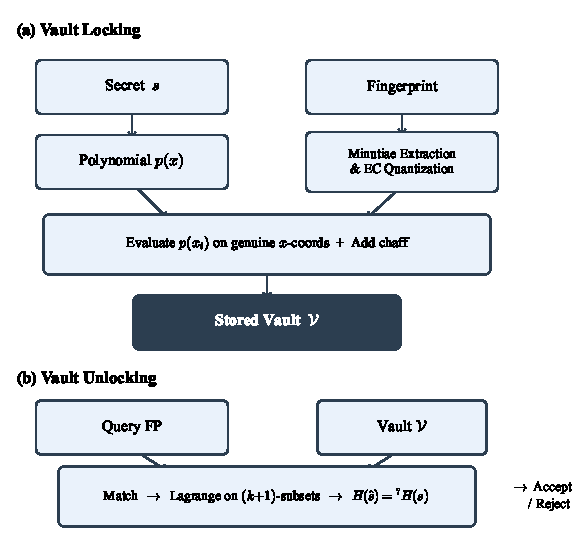
\includegraphics[width=\columnwidth]{figures/fig_fuzzy_vault_concept.pdf}
    \caption{Fuzzy vault concept: (a)~Locking phase---genuine points lie on secret polynomial $p(x)$, chaff points are randomly scattered. (b)~Unlocking phase---query matches identify candidate genuine points for Lagrange interpolation.}
    \label{fig:fuzzy_vault_concept}
\end{figure}

\subsection{ECC-Based Fuzzy Vault}
\label{sec:ecc_vault}

We adopt the ECC vault construction of~\cite{maurya2025enhancing}. Let $E$ be the Brainpool~P256r1 elliptic curve over $\GFp{}$ with generator $G$ and prime order $n$.

\subsubsection{Locking (Enrollment)}
Given a set of fingerprint minutiae $\mathcal{M} = \{m_1, \ldots, m_t\}$, the vault is constructed as follows:

\begin{enumerate}
    \item \textbf{Quantization}: Each minutia $m_i = (x_i, y_i, \theta_i)$ is quantized by a factor $f$: $q_i = (\lfloor x_i/f \rfloor \bmod 64) \| (\lfloor y_i/f \rfloor \bmod 64) \| (\lfloor \theta_i/f \rfloor \bmod 64)$, producing an 18-bit integer. Duplicate quantized values are removed, yielding $\mathcal{Q} = \{q_1, \ldots, q_g\}$ with $g \leq t$.
    \item \textbf{EC Mapping}: Each $q_i$ is mapped to an EC point $P_i = q_i \cdot G$, a one-way mapping protected by ECDLP.
    \item \textbf{Polynomial Generation}: A random polynomial $p(x) = \sum_{j=0}^{k} a_j x^j$ of degree $k$ is generated over $\GFp{}$, with coefficients $a_j \in [10, 63]$ (6 bits each). The secret key is $s = \left(\bigoplus_{j=0}^{k} \text{bin}_6(a_j)\right) \bmod n$, and the public key is $S = s \cdot G$.
    \item \textbf{Genuine Point Projection}: Each genuine minutia is projected onto the polynomial: $\mathcal{G} = \{(P_i.x, \; p(P_i.x))\}_{i=1}^{g}$.
    \item \textbf{Chaff Generation}: $5g$ chaff points are generated: $\mathcal{C} = \{(c_j.x, r_j)\}_{j=1}^{5g}$ where $r_j \neq p(c_j.x)$, \ie{}, chaff points do \emph{not} lie on $p(x)$.
    \item \textbf{Vault Assembly}: All $6g$ points are randomly shuffled: $\mathcal{V} = \text{shuffle}(\mathcal{G} \cup \mathcal{C})$. The vault stores $(\mathcal{V}, S)$.
\end{enumerate}

The security of the vault relies on the indistinguishability of genuine and chaff points: without knowing which points lie on $p(x)$, an adversary must try $\binom{6g}{k+1}$ subsets.

\subsubsection{Unlocking (Verification)}
Given query minutiae $\mathcal{M}'$, quantize to $\mathcal{Q}'$ and find matching x-coordinates $\mathcal{X}_m = \{x : (x,y) \in \mathcal{V}, \exists q' \in \mathcal{Q}' \text{ s.t. } (q' \cdot G).x = x\}$. If $|\mathcal{X}_m| \geq k+1$, for each $(k{+}1)$-subset of $\mathcal{X}_m$, perform Lagrange interpolation to reconstruct a candidate polynomial $\hat{p}(x)$, compute $\hat{s}$, and verify $\hat{s} \cdot G \stackrel{?}{=} S$. The vault is successfully unlocked if any subset yields a matching public key.

\subsection{Iris Code Extraction Pipeline}
\label{sec:iris_extraction}

We implement a custom iris recognition pipeline following Daugman~\cite{daugman2004how} and Masek~\cite{masek2003thesis}. The pipeline operates on $320 \times 280$ near-infrared (NIR) images from CASIA-Iris-Interval.

\subsubsection{Segmentation}
Pupil detection is performed by thresholding (intensity $< 70$) on the NIR image after inpainting LED specular reflections. The pupil boundary is refined via contour analysis, with fallback to the Hough Circle Transform for low-contrast images. The iris outer boundary is located using an integrodifferential-style operator: we compute the mean intensity on concentric circles at increasing radii from the pupil center, take the radial derivative, smooth with a Gaussian kernel, and select the radius with maximum gradient response. A noise mask excludes regions outside the iris, the pupil interior, and specular reflections (intensity $> 210$). Eyelid occlusions are detected using a column-by-column intensity variance analysis on the normalized strip: for each column, a sliding-window variance profile is computed and the row with maximum variance (indicating the texture transition between eyelid skin and iris stroma) is identified independently in the upper and lower halves. Rows beyond the detected transition boundary are masked. This approach avoids parametric eyelid models (e.g., parabolic or elliptical fits) and adapts to non-standard eyelid geometries.

\subsubsection{Normalization}
The annular iris region is unwrapped to a fixed $64 \times 512$ rectangular strip using Daugman's rubber-sheet model, which maps each point $(r, \theta)$ in the iris annulus to a Cartesian coordinate in the normalized image, handling non-concentric pupil and iris centers. The noise mask is simultaneously remapped.

\subsubsection{Encoding}
The normalized strip is contrast-enhanced using CLAHE (Contrast-Limited Adaptive Histogram Equalization) and encoded using 1D Log-Gabor filters applied in the frequency domain (FFT-based) at two center wavelengths (18 and 36~pixels), with a bandwidth parameter of $\sigma/f = 0.30$. All 64 rows of the normalized strip are encoded; eyelid and occlusion contamination is handled entirely by the validity mask (see Segmentation above) rather than by row exclusion. The complex filter response is phase-quantized into 2 bits per position (sign of real and imaginary parts), following the standard Daugman encoding. Fragile bits---those near phase boundaries where the filter response amplitude falls below 0.55$\times$ the median---are masked out~\cite{hollingsworth2009fragile}. The resulting iris code has $64 \times 512 \times 2 \times 2 = 131{,}072$ bits with an associated validity mask (mean coverage $\approx 26\%$).

\subsubsection{Matching}
Iris codes are compared using fractional Hamming distance (FHD), computed only over mutually valid bits. Circular bit-shifts ($\pm 32$ columns $\times$ 512-pixel rows) compensate for rotational misalignment, and the minimum FHD across all shifts is taken as the final distance. 

\subsection{Iris Fuzzy Commitment with Bit Interleaving}
\label{sec:iris_commitment}

We extract a stable binary key from iris codes using a repetition-code fuzzy commitment. Let $\mathbf{c} \in \{0,1\}^{N}$ denote an $N$-bit iris code ($N = 131{,}072$ in our implementation) and let $B_s$ denote the \emph{block size} (number of bits per block). The number of blocks is $n_b = \lfloor N / B_s \rfloor$, each contributing one key bit, yielding an $n_b$-bit key.

\subsubsection{Enrollment}
\begin{enumerate}
    \item Partition the code into $n_b$ blocks using \emph{interleaved} assignment: bit $j$ belongs to block $(j \bmod n_b)$, distributing spatially correlated errors across blocks rather than concentrating them in contiguous regions.
    \item Generate a random $n_b$-bit key $\mathbf{k} = (k_0, \ldots, k_{n_b-1})$.
    \item Construct a repetition codeword $\mathbf{w}$: position $j$ is set to $k_{j \bmod n_b}$.
    \item Compute helper data $\mathbf{h} = \mathbf{c} \oplus \mathbf{w}$ and store $(\mathbf{h}, H(\mathbf{k}))$ where $H$ is SHA-256.
\end{enumerate}

\subsubsection{Recovery}
Given query code $\mathbf{c}'$, for each rotation shift $\delta \in [-32, +32]$ (compensating for head tilt):
\begin{enumerate}
    \item Compute $\tilde{\mathbf{c}} = \text{rotate}(\mathbf{c}', \delta)$ and $\tilde{\mathbf{w}} = \tilde{\mathbf{c}} \oplus \mathbf{h}$.
    \item For each block $i$, recover $\hat{k}_i$ by majority vote over the block's valid positions (excluding masked bits). With $B_s = 255$, the error correction capacity per block is $(B_s - 1)/2 = 127$ bit errors (up to 49.8\% error rate per block). Since genuine iris pairs exhibit FHD~$\approx 0.20$ (i.e., $\sim$51 errors per 255-bit block on average), majority vote succeeds for most blocks; however, all $n_b = 514$ blocks must decode correctly for key recovery, yielding an overall GAR of $\sim$62\%.
    \item If $H(\hat{\mathbf{k}}) = H(\mathbf{k})$, recovery succeeds; return $\hat{\mathbf{k}}$.
\end{enumerate}

% ============================================================================
% IV. PROPOSED ARCHITECTURE: IBFV
% ============================================================================
\section{Proposed Architecture: \IBFV{}}
\label{sec:proposed}

\subsection{Motivation: The AND-Fusion Penalty}
\label{sec:motivation}

Consider a conventional multimodal fuzzy vault where the iris is used as a mandatory gate (\eg{}, Architecture~A in our experiments). Let $\GAR_{\text{FP}}$ and $\GAR_{\text{Iris}}$ denote the genuine acceptance rates of the fingerprint and iris subsystems, respectively. Under AND-fusion:
\begin{equation}
    \GAR_{\text{AND}} = \GAR_{\text{FP}} \times \GAR_{\text{Iris}} \leq \GAR_{\text{FP}}
    \label{eq:and_penalty}
\end{equation}
Since $\GAR_{\text{Iris}} < 1$ in practice (our measurements show $\GAR_{\text{Iris}} \approx 62\%$ for Setup~1), the AND-fusion GAR in~(\ref{eq:and_penalty}) is \emph{always} lower than the unimodal fingerprint GAR. For a system where the unimodal FRR is already low, this penalty is devastating. Fig.~\ref{fig:and_vs_ibfv} illustrates the fundamental difference between AND-fusion (gating) and \IBFV{} (boosting).

\begin{figure}[t]
    \centering
    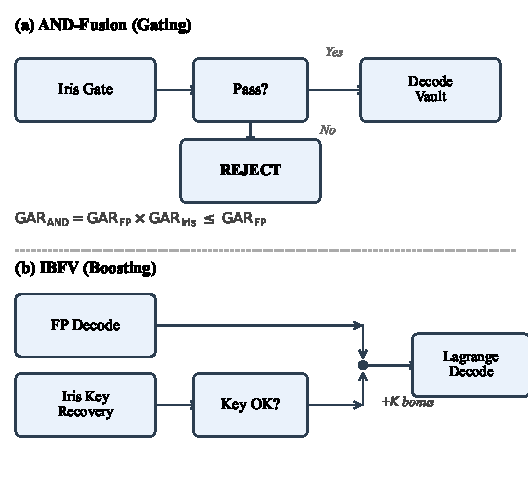
\includegraphics[width=\columnwidth]{figures/fig_and_vs_ibfv.pdf}
    \caption{AND-fusion vs.\ \IBFV{}: (a)~AND-fusion uses the iris as a mandatory gate---38\% of genuine users are blocked regardless of fingerprint quality. (b)~\IBFV{} uses the iris as an optional booster---no genuine user is ever worse off.}
    \label{fig:and_vs_ibfv}
\end{figure}

\subsection{IBFV Enrollment}
\label{sec:ibfv_enrollment}

Given fingerprint minutiae $\mathcal{M}$ and iris code $(\mathbf{c}, \mathbf{mask})$, the enrollment procedure (Algorithm~\ref{alg:enrollment}, Fig.~\ref{fig:ibfv_enrollment}) proceeds as follows:

\begin{enumerate}
    \item Execute the standard ECC vault enrollment (Section~\ref{sec:ecc_vault}) to obtain genuine points $\mathcal{G}_{\text{FP}}$, polynomial $p(x)$, and public key $S$.
    \item Perform iris fuzzy commitment enrollment (Section~\ref{sec:iris_commitment}) with block size $B_s$ to obtain commitment $(\mathbf{h}, H(\mathbf{k}))$ and key hash $\kappa = H(\mathbf{k})$.
    \item \textbf{Derive virtual x-coordinates}: For $j = 0, \ldots, K{-}1$:
    \begin{equation}
        v_j = \text{SHA-256}\!\left(\texttt{"ibfv\_vpt:"} \| j \| \texttt{":"} \| \kappa\right) \bmod p
        \label{eq:virtual_x}
    \end{equation}
    ensuring $v_j \notin \{P_i.x : P_i \in \mathcal{G}_{\text{FP}}\}$ and $v_j \neq v_\ell$ for $j \neq \ell$.
    \item \textbf{Compute bonus points}: $\mathcal{G}_{\text{Iris}} = \{(v_j, p(v_j))\}_{j=0}^{K-1}$.
    \item \textbf{Generate chaff}: $5|\mathcal{G}_{\text{FP}}|$ chaff points (chaff count based on fingerprint points only).
    \item \textbf{Construct vault}: $\mathcal{V} = \text{shuffle}(\mathcal{G}_{\text{FP}} \cup \mathcal{G}_{\text{Iris}} \cup \mathcal{C})$.
\end{enumerate}

The stored vault is $(\mathcal{V}, S, \mathbf{h}, H(\mathbf{k}), B_s)$.

\begin{figure}[t]
    \centering
    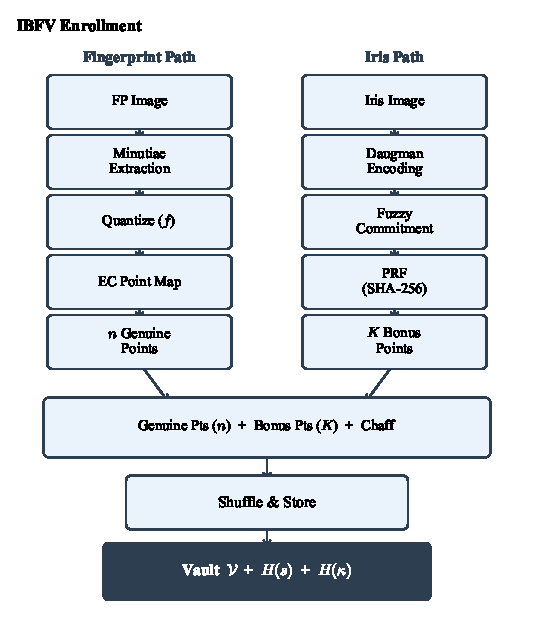
\includegraphics[width=\columnwidth]{figures/fig_ibfv_enrollment.pdf}
    \caption{\IBFV{} enrollment pipeline. The fingerprint path produces genuine vault points via EC mapping onto Brainpool~P256r1. The iris path extracts a stable key via fuzzy commitment, which seeds a PRF to derive $K$ bonus polynomial points. All points are merged with chaff and shuffled into the final vault.}
    \label{fig:ibfv_enrollment}
\end{figure}

\begin{algorithm}[t]
\caption{\IBFV{} Enrollment}
\label{alg:enrollment}
\begin{algorithmic}[1]
\REQUIRE Minutiae $\mathcal{M}$, iris code $(\mathbf{c}, \mathbf{mask})$, params $(f, k, K, B_s)$
\ENSURE Vault $(\mathcal{V}, S, \mathbf{h}, H(\mathbf{k}), B_s)$
\STATE $\mathcal{Q} \leftarrow \textsc{Quantize}(\mathcal{M}, f)$
\STATE $\{P_i\} \leftarrow \{q \cdot G : q \in \mathcal{Q}\}$ \COMMENT{EC mapping}
\STATE $p(x) \leftarrow$ random degree-$k$ polynomial over $\GFp{}$
\STATE $s \leftarrow \text{bin}(p) \bmod n$; $S \leftarrow s \cdot G$
\STATE $\mathcal{G}_\text{FP} \leftarrow \{(P_i.x,\; p(P_i.x))\}_{i=1}^{g}$
\STATE $(\mathbf{h}, \kappa) \leftarrow \textsc{IrisEnroll}(\mathbf{c}, \mathbf{mask}, B_s)$
\FOR{$j = 0$ \TO $K{-}1$}
    \STATE $v_j \leftarrow \text{SHA256}(\texttt{"ibfv\_vpt:"} \| j \| \texttt{":"} \| \kappa) \bmod p$
\ENDFOR
\STATE $\mathcal{G}_\text{Iris} \leftarrow \{(v_j,\; p(v_j))\}_{j=0}^{K-1}$
\STATE $\mathcal{C} \leftarrow \textsc{GenChaff}(5g)$ \COMMENT{$5\times$ FP count}
\STATE $\mathcal{V} \leftarrow \textsc{Shuffle}(\mathcal{G}_\text{FP} \cup \mathcal{G}_\text{Iris} \cup \mathcal{C})$
\RETURN $(\mathcal{V}, S, \mathbf{h}, \kappa, B_s)$
\end{algorithmic}
\end{algorithm}

\subsection{IBFV Verification}
\label{sec:ibfv_verification}

Given query fingerprint $\mathcal{M}'$ and iris code $(\mathbf{c}', \mathbf{mask}')$, verification (Algorithm~\ref{alg:verification}, Fig.~\ref{fig:ibfv_verification}) proceeds:

\begin{enumerate}
    \item Quantize query minutiae → find FP-matching vault points: $\mathcal{X}_{\text{FP}} = \{(x,y) \in \mathcal{V} : x \in \text{EC}(\mathcal{Q}')\}$.
    \item Attempt iris key recovery (Section~\ref{sec:iris_commitment}).
    \item \textbf{If iris succeeds} (key $\hat{\mathbf{k}}$ recovered):
    \begin{enumerate}
        \item Derive virtual x-coordinates $\{v_0, \ldots, v_{K-1}\}$ using~(\ref{eq:virtual_x}).
        \item Find bonus matches: $\mathcal{X}_{\text{Iris}} = \{(x,y) \in \mathcal{V} : x \in \{v_j\}\}$.
        \item Total candidate set: $\mathcal{X} = \mathcal{X}_{\text{FP}} \cup \mathcal{X}_{\text{Iris}}$.
        \item \textbf{Smart decoding}: Try $(k{+}1)$-subsets of $\mathcal{X}$ that include \emph{all} $K$ bonus points first (since these are guaranteed genuine), reducing the search from $\binom{|\mathcal{X}|}{k+1}$ to $\binom{|\mathcal{X}_{\text{FP}}|}{k+1-K}$.
    \end{enumerate}
    \item \textbf{If iris fails}: Set $\mathcal{X} = \mathcal{X}_{\text{FP}}$ and proceed with standard Lagrange interpolation---identical to the unimodal vault.
\end{enumerate}

\noindent\textbf{Complexity reduction.} The smart decoding strategy exploits the fact that all $K$ bonus points are \emph{guaranteed genuine} (they were derived from the correct iris key). Instead of enumerating all $\binom{|\mathcal{X}|}{k+1}$ subsets, the decoder fixes the $K$ bonus points and selects only the remaining $k+1-K$ points from the fingerprint candidate set $\mathcal{X}_{\text{FP}}$. This reduces the search space by a factor of:
\begin{equation}
    \frac{\binom{|\mathcal{X}_{\text{FP}}| + K}{k+1}}{\binom{|\mathcal{X}_{\text{FP}}|}{k+1-K}}
    \label{eq:complexity_reduction}
\end{equation}
For typical parameters ($|\mathcal{X}_{\text{FP}}| = 12$, $k = 10$, $K = 4$), this ratio is $\binom{16}{11}/\binom{12}{7} = 4368/792 = 5.5\times$, yielding a proportional speed-up in verification time while simultaneously \emph{increasing} the probability of selecting a valid $(k{+}1)$-subset.

\begin{algorithm}[t]
\caption{\IBFV{} Verification}
\label{alg:verification}
\begin{algorithmic}[1]
\REQUIRE Query $(\mathcal{M}', \mathbf{c}', \mathbf{mask}')$, vault $(\mathcal{V}, S, \mathbf{h}, \kappa, B_s)$
\ENSURE Accept / Reject
\STATE $\mathcal{Q}' \leftarrow \textsc{Quantize}(\mathcal{M}', f)$
\STATE $\mathcal{X}_\text{FP} \leftarrow \{(x,y) \in \mathcal{V} : x \in \text{EC}(\mathcal{Q}')\}$
\STATE $\hat{\mathbf{k}} \leftarrow \textsc{IrisRecover}(\mathbf{c}', \mathbf{mask}', \mathbf{h}, \kappa, B_s)$
\IF{$\hat{\mathbf{k}} \neq \bot$}
    \FOR{$j = 0$ \TO $K{-}1$}
        \STATE $v_j \leftarrow \text{SHA256}(\texttt{"ibfv\_vpt:"} \| j \| \texttt{":"} \| H(\hat{\mathbf{k}})) \bmod p$
    \ENDFOR
    \STATE $\mathcal{X}_\text{Iris} \leftarrow \{(x,y) \in \mathcal{V} : x \in \{v_j\}\}$
    \STATE $\mathcal{X} \leftarrow \mathcal{X}_\text{FP} \cup \mathcal{X}_\text{Iris}$
\ELSE
    \STATE $\mathcal{X} \leftarrow \mathcal{X}_\text{FP}$ \COMMENT{Fallback: no penalty}
\ENDIF
\FOR{each $(k{+}1)$-subset $\mathcal{S} \subseteq \mathcal{X}$}
    \STATE $\hat{p} \leftarrow \textsc{LagrangeInterp}(\mathcal{S})$
    \STATE $\hat{s} \leftarrow \text{bin}(\hat{p}) \bmod n$
    \IF{$\hat{s} \cdot G = S$}
        \RETURN \textbf{Accept}
    \ENDIF
\ENDFOR
\RETURN \textbf{Reject}
\end{algorithmic}
\end{algorithm}

\begin{figure}[t]
    \centering
    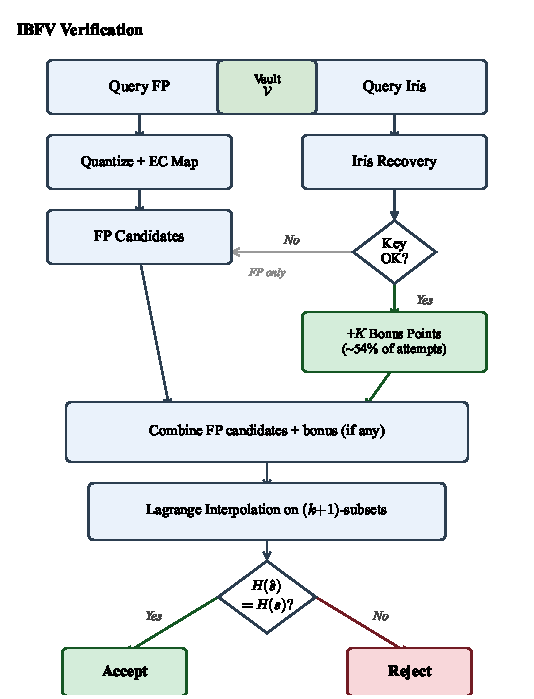
\includegraphics[width=\columnwidth]{figures/fig_ibfv_verification.pdf}
    \caption{\IBFV{} verification pipeline. If iris key recovery succeeds ($\sim$62\% of genuine attempts), $K$ bonus points are added to the candidate set, strictly reducing the combinatorial search space. If it fails ($\sim$38\%), the system degrades to unimodal fingerprint decoding with \emph{zero penalty}. Dashed paths denote the fallback (iris-failure) branch.}
    \label{fig:ibfv_verification}
\end{figure}

\subsection{Zero-Penalty Theorem}
\label{sec:zero_penalty}

\begin{theorem}[Zero-Penalty Guarantee]
\label{thm:zero_penalty}
For any parameter configuration $(f, k)$ and any biometric sample pair $(\mathcal{M}', \mathbf{c}')$, the \IBFV{} verification outcome satisfies:
\begin{equation}
    \Pr[\text{Accept}_{\IBFV}] \geq \Pr[\text{Accept}_{\text{Uni}}]
\end{equation}
where the probability is over the randomness in vault construction.
\end{theorem}

\begin{proof}
The \IBFV{} verification process has two exclusive branches:
\begin{itemize}
    \item \textbf{Iris succeeds}: The candidate set $|\mathcal{X}| = |\mathcal{X}_{\text{FP}}| + K \geq |\mathcal{X}_{\text{FP}}|$, and all $K$ bonus points are on the polynomial. Since the unimodal decoder receives only $\mathcal{X}_{\text{FP}}$ while \IBFV{} receives $\mathcal{X}_{\text{FP}} \cup \mathcal{X}_{\text{Iris}}$, every $(k{+}1)$-subset available to the unimodal decoder is also available to \IBFV{}, plus additional subsets containing bonus points. If the unimodal decoder accepts, so does \IBFV{}.
    \item \textbf{Iris fails}: The fallback path uses $\mathcal{X} = \mathcal{X}_{\text{FP}}$ with identical Lagrange interpolation, producing the same outcome as the unimodal decoder.
\end{itemize}
In neither case does \IBFV{} reject when the unimodal decoder would accept. \qed
\end{proof}

\begin{corollary}
$\FRR_{\IBFV} \leq \FRR_{\text{Uni}}$ for all $(f,k)$. If the iris impostor acceptance rate is zero, bonus points are never injected for impostors, so $\FAR_{\IBFV} \leq \FAR_{\text{Uni}}$ and therefore $\EER_{\IBFV} \leq \EER_{\text{Uni}}$. In practice at $B_s = 255$, the iris impostor FAR is $\sim$0.10\% (Section~\ref{sec:iris_gar_results}), so a small fraction of impostors receive bonus points, potentially elevating $\FAR_{\IBFV}$ above $\FAR_{\text{Uni}}$ by up to 0.07~pp on easy databases. The EER guarantee holds exactly when the iris impostor FAR is zero, and approximately when it is near-zero.
\end{corollary}

% ============================================================================
% V. SECURITY ANALYSIS
% ============================================================================
\section{Security Analysis}
\label{sec:security}

We analyze the \IBFV{} scheme against the ISO/IEC 24745~\cite{iso24745} requirements for biometric template protection: irreversibility, unlinkability, and revocability. We adopt the adversary model of Ratha~\textit{et~al.}~\cite{ratha2001enhancing}, which identifies eight attack points in a generic biometric authentication system.

\subsection{Threat Model}
\label{sec:threat_model}

Following Ratha~\textit{et~al.}~\cite{ratha2001enhancing}, we consider eight attack points in the biometric pipeline (see Fig.~\ref{fig:threat_model}):

\begin{figure*}[t]
    \centering
    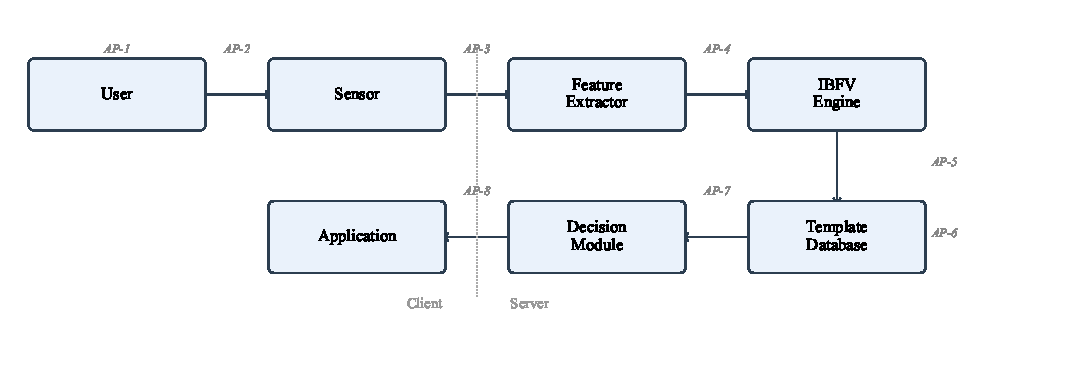
\includegraphics[width=\textwidth]{figures/fig_threat_model.pdf}
    \caption{Threat model: eight attack points (AP-1 through AP-8) in the \IBFV{} biometric pipeline, following Ratha~\textit{et~al.}~\cite{ratha2001enhancing}. The primary threat (AP-6, database breach) is the focus of our security analysis; other attack points are mitigated by standard measures as annotated.}
    \label{fig:threat_model}
\end{figure*}

\begin{enumerate}
    \item \textbf{Spoofing (AP-1)}: Presenting a fake biometric (artificial finger, printed iris). \emph{Countermeasure}: Liveness detection---outside the scope of template protection but complementary.
    \item \textbf{Sensor-to-extractor interception (AP-2)}: Replaying a captured raw image. \emph{Countermeasure}: Client-side processing; channel assumed secure.
    \item \textbf{Feature extractor compromise (AP-3)}: Trojan horse in the extraction module. \emph{Countermeasure}: Trusted computing base; client-side integrity assumed.
    \item \textbf{Feature channel interception (AP-4)}: Intercepting extracted features in transit. \emph{Countermeasure}: All processing is local---no feature transmission.
    \item \textbf{Matcher/engine compromise (AP-5)}: Hill-climbing or perturbation attacks using match scores. \emph{Countermeasure}: The \IBFV{} decoder outputs only a binary Accept/Reject decision---no confidence scores are exposed, eliminating the gradient signal required for hill-climbing~\cite{ratha2001enhancing}.
    \item \textbf{Database breach (AP-6)} {\bfseries [Primary threat]}: The adversary obtains the stored template $(\mathcal{V}, S, \mathbf{h}, H(\mathbf{k}), B_s)$ in its entirety. This is the central threat model for BTP schemes. We address this in Sections~\ref{sec:irreversibility}--\ref{sec:brute_force}.
    \item \textbf{Database-to-engine channel (AP-7)}: Replaying vault data during verification. \emph{Countermeasure}: The vault alone cannot authenticate without a live biometric query to produce matching points.
    \item \textbf{Decision override (AP-8)}: Flipping the Accept/Reject decision. \emph{Countermeasure}: Standard transport-layer security (TLS/mTLS)---system-level, not template-level.
\end{enumerate}

We assume the adversary has full access to the stored template (AP-6) and the iris helper data, but does not possess the original biometric samples. This is the standard ``stolen-token'' model for template protection evaluation.

\subsection{Irreversibility (Non-Invertibility)}
\label{sec:irreversibility}

We establish that three independent barriers prevent template inversion.

\subsubsection{Fingerprint Recovery from Vault}
Given vault $\mathcal{V}$ containing $g$ genuine and $5g + K$ non-genuine points, the adversary must identify the genuine subset. Without knowledge of which points lie on the polynomial $p(x)$, the adversary faces a combinatorial identification problem. Even after identifying $k+1$ genuine points, recovering the original minutiae requires inverting the EC mapping: given $P_i.x$, finding $q_i$ such that $(q_i \cdot G).x = P_i.x$ is an instance of ECDLP.

For Brainpool~P256r1 with a 256-bit group order, the best known attack (Pollard's rho method) requires approximately:
\begin{equation}
    \sqrt{\pi n / 2} \approx 2^{128} \text{ group operations}
    \label{eq:ecdlp_cost}
\end{equation}
At $10^9$ operations per second, this requires approximately $10^{29}$ seconds ($\sim\! 3 \times 10^{21}$ years), providing a wide margin above the $2^{80}$ threshold typically considered infeasible.

\subsubsection{Iris Code Recovery}
The helper data $\mathbf{h} = \mathbf{c} \oplus \mathbf{w}$ reveals no information about the iris code $\mathbf{c}$ without knowing the codeword $\mathbf{w}$. The space of valid codewords is $\{0,1\}^{n_b}$ (repeated to length $N$), giving $2^{n_b}$ possibilities. For $B_s = 255$ (giving $n_b = \lfloor 131072/255 \rfloor = 514$ key bits), the brute-force cost is $2^{514} \approx 10^{155}$ hash evaluations---completely infeasible.

\subsubsection{Bonus Point Identification}
Without the iris key hash $\kappa = H(\mathbf{k})$, the adversary cannot compute the virtual x-coordinates~(\ref{eq:virtual_x}) due to the preimage resistance of SHA-256. The $K$ bonus points are computationally indistinguishable from chaff and genuine fingerprint points in $\GFp{}$, as they are uniformly distributed 256-bit integers (by the PRF property of SHA-256). This adds $K$ additional unknowns to the vault identification problem.

\subsection{Unlinkability}
\label{sec:unlinkability}

Given two vaults $\mathcal{V}_1, \mathcal{V}_2$ enrolled from the same user in different applications, unlinkability requires that no polynomial-time adversary can determine whether the vaults share a common biometric source.

\IBFV{} achieves unlinkability through three independent mechanisms:
\begin{enumerate}
    \item \textbf{Random polynomial}: Each enrollment uses an independently sampled polynomial $p(x)$, so the $y$-coordinates $(p(P_i.x))$ are statistically independent across enrollments.
    \item \textbf{Random chaff}: Chaff points are uniformly generated in each enrollment, providing no cross-vault correlation.
    \item \textbf{Iris-derived coordinates}: The virtual x-coordinates $\{v_j\}$ depend on $\kappa = H(\mathbf{k})$, which is deterministic per enrollment. However, if different applications use different quantization/commitment parameters (standard practice for revocability), the resulting $\kappa$ values differ, producing independent PRF outputs.
\end{enumerate}

\noindent While the \emph{genuine x-coordinates} repeat across enrollments (since they derive from the same biometric), these are hidden among $5g + K$ non-genuine points. Identifying common genuine points across two vaults requires solving the intersection problem on shuffled sets---equivalent to the polynomial reconstruction attack, which is combinatorially hard (Section~\ref{sec:brute_force}).

\subsection{Revocability}
\label{sec:revocability}

If a vault is compromised, the user re-enrolls with a new random polynomial, new random seed for quantization (\eg{}, different factor $f$ or domain-specific salt), and a fresh iris commitment (using a different random key $\mathbf{k}'$). The new vault's genuine point projections $p'(P_i.x)$, chaff, and iris-derived bonus coordinates are all independent of the revoked vault. Multiple revocations are supported without biometric re-acquisition---only the computational parameters change.

\subsection{Brute-Force Attack Analysis}
\label{sec:brute_force}

We quantify the computational cost of a brute-force attack on a stolen vault.

\subsubsection{Polynomial Reconstruction Attack}
The adversary must identify at least $k+1$ genuine points among $|\mathcal{V}| = 6g + K$ total points. With typical parameters ($g \approx 20$, $K = 4$, $k = 10$), the vault contains $6(20) + 4 = 124$ points, of which $20 + 4 = 24$ are genuine. The number of candidate $(k+1)$-subsets is:
\begin{equation}
    \binom{124}{k+1} = \binom{124}{11} \approx 1.7 \times 10^{15}
    \label{eq:brute_force}
\end{equation}
Each candidate requires one Lagrange interpolation (${O}(k^2)$ field operations) and one EC scalar multiplication ($\hat{s} \cdot G$, approximately 256 point additions). At $10^6$ candidates evaluated per second, exhaustive search requires:
\begin{equation}
    \frac{1.7 \times 10^{15}}{10^6} \approx 1.7 \times 10^{9} \text{ seconds} \approx 54 \text{ years}
\end{equation}

However, the adversary need not try all subsets; success is expected after trying approximately $\binom{124}{11} / \binom{24}{11}$ subsets (since each genuine $(k+1)$-subset succeeds). This gives:
\begin{equation}
    \frac{\binom{124}{11}}{\binom{24}{11}} = \frac{1.7 \times 10^{15}}{2.5 \times 10^{6}} \approx 6.8 \times 10^{8} \text{ attempts}
\end{equation}
At $10^6$ attempts/second, this requires $\sim\!680$ seconds---\emph{feasible} for an offline attacker who possesses $S$. This is a well-known limitation shared by all fuzzy vault schemes where the public key is stored alongside the vault~\cite{tams2013attacks,nandakumar2007fuzzy}. Standard mitigations include: (1)~storing $S$ in a separate security domain (e.g., a hardware security module) so that vault compromise alone is insufficient; (2)~increasing the polynomial degree $k$ (at $k = 15$, the cost rises to $\binom{124}{16} \approx 10^{20}$, requiring $\sim\!3 \times 10^{6}$ years); and (3)~adding a key-stretching function (e.g., Argon2) to the verification operation to increase per-attempt cost. We note that the primary template protection goal---preventing \emph{biometric recovery}---is achieved regardless, since reconstructing $p(x)$ reveals only the secret $s$, not the original minutiae (which requires solving ECDLP as per Section~\ref{sec:irreversibility}).

\subsubsection{Comparison with Unimodal Vault}
Without \IBFV{} bonus points, $K = 0$ and the vault has $6 \times 20 = 120$ points with 20 genuine. The IBFV vault ($6 \times 20 + 4 = 124$ points, 24 genuine) increases the total vault size but also increases the genuine fraction from $20/120 = 16.7\%$ to $24/124 = 19.4\%$, slightly increasing the probability of randomly selecting a genuine point.

However, the \emph{effective security} increases because: (1) the bonus points are unknown to an adversary without $\kappa$, adding $K$ extra unknowns; and (2) the genuine-to-chaff ratio for the fingerprint subset alone remains unchanged at $g/(5g) = 1/5$. The improved genuine fraction comes entirely from the cryptographically protected bonus points, which provide no exploitable structure.

\subsection{Cross-Matching Attack}
\label{sec:cross_matching}

In a cross-matching attack~\cite{tams2013attacks}, the adversary possesses vaults from two different applications enrolled with the same biometric and attempts to correlate them to determine if they belong to the same user. The adversary compares x-coordinate sets across vaults to find common genuine points.

In \IBFV{}, the genuine fingerprint x-coordinates are deterministic (derived from the same minutiae), so they appear in both vaults. However, these are hidden among $5g$ random chaff points per vault. The probability that a chaff point in vault 1 coincidentally matches a chaff point in vault 2 (in a 256-bit field) is $1/p \approx 2^{-256}$ per pair---negligible.

\emph{Countermeasure}: Using different quantization parameters ($f_1 \neq f_2$) across applications produces different quantized values, different EC mappings, and therefore different genuine x-coordinates. This eliminates the cross-matching signal entirely. We recommend application-specific parameters as standard practice for multi-application deployments.

\subsection{Formal Unlinkability Analysis ($D_{\text{sys}}$)}
\label{sec:dsys}

To complement the theoretical arguments above, we empirically evaluate unlinkability using the $D_{\text{sys}}$ metric of Gomez-Barrero~\textit{et~al.}~\cite{gomezbarrero2017}. This framework measures the degree to which an adversary can distinguish mated (same-subject) from non-mated (different-subject) template pairs based on their similarity, yielding a score $D_{\text{sys}} \in [0, 1]$ where $0$ indicates fully unlinkable and $1$ indicates fully linkable.

We construct vault pairs under three scenarios for each database (Setup~1):
\begin{itemize}
    \item \textbf{Same-factor}: Both vaults use identical quantization parameters $(f, k)$---the worst case for unlinkability, as genuine x-coordinates repeat.
    \item \textbf{Different-factor}: Vaults use different factors ($f_1 \neq f_2$, same $k$)---the recommended deployment configuration.
    \item \textbf{Diverse-factor}: Vaults use substantially different parameters ($f_1$ and $f_2$ far apart)---simulating distinct applications.
\end{itemize}

Mated and non-mated similarity is quantified by the number of matching x-coordinates between vault pairs. Table~\ref{tab:dsys} reports the $D_{\text{sys}}$ values.

\begin{table}[t]
\centering
\caption{Unlinkability: $D_{\text{sys}}$ metric (lower is better; $D_{\text{sys}} = 0$ is fully unlinkable, $D_{\text{sys}} = 1$ is fully linkable).}
\label{tab:dsys}
\begin{tabular}{@{}l c c c c@{}}
\toprule
\textbf{Scenario} & \textbf{DB1} & \textbf{DB2} & \textbf{DB3} & \textbf{DB4} \\
\midrule
Same-factor     & 0.994 & 0.994 & 0.920 & 0.929 \\
Different-factor & 0.317 & 0.313 & 0.057 & 0.388 \\
Diverse-factor   & 0.003 & 0.014 & 0.026 & 0.007 \\
\bottomrule
\end{tabular}
\end{table}

As expected, same-factor enrollments are highly linkable ($D_{\text{sys}} > 0.92$) because the deterministic genuine x-coordinates repeat. However, changing the quantization factor---the standard revocability practice---dramatically reduces linkability: different-factor $D_{\text{sys}} \leq 0.39$, and diverse-factor $D_{\text{sys}} \leq 0.03$. In the recommended deployment configuration (application-specific parameters), \IBFV{} achieves near-perfect unlinkability, empirically confirming the theoretical argument from Section~\ref{sec:unlinkability}.

\subsection{Vault Entropy}
\label{sec:vault_entropy}

The genuine x-coordinates are EC point x-coordinates in $\GFp{}$, where $p$ is a 256-bit prime. With Shannon entropy $H \geq 7.7$ bits and min-entropy $H_\infty \geq 5.9$ bits per coordinate (Section~\ref{sec:entropy_results}), the vault provides substantial resistance against dictionary attacks. The per-user KL divergence from uniform is $\leq 0.32$ bits, and the genuine-vs-chaff KL divergence is $\approx 0.24$ bits across all databases, indicating near-uniform mixing---an adversary cannot distinguish genuine from chaff points based on their x-coordinate distribution alone.

% ============================================================================
% VI. EXPERIMENTAL RESULTS
% ============================================================================
\section{Experimental Results}
\label{sec:experiments}

\subsection{Databases and Configuration}
\label{sec:databases}

\subsubsection{Fingerprint Databases}
We evaluate on four FVC benchmark databases:
\begin{itemize}
    \item \textbf{DB1} (FVC2002 DB1)~\cite{maio2002fvc2002}: 100 subjects $\times$ 8 impressions, optical sensor.
    \item \textbf{DB2} (FVC2002 DB2)~\cite{maio2002fvc2002}: 100 subjects $\times$ 8 impressions, capacitive sensor.
    \item \textbf{DB3} (FVC2002 DB3)~\cite{maio2002fvc2002}: 100 subjects $\times$ 8 impressions, thermal sweep sensor. Known for low quality.
    \item \textbf{DB4} (FVC2004 DB1)~\cite{maio2004fvc2004}: 100 subjects $\times$ 8 impressions, optical sensor with deliberate difficulty.
\end{itemize}

\subsubsection{Iris Database}
CASIA-Iris-Interval~\cite{casia_iris}: 249 subjects $\times$ multiple captures under near-infrared illumination (1329/1332 images successfully processed, 99.8\% extraction rate). Since no publicly available dataset contains co-acquired fingerprint and iris samples from the same subjects, we construct a \emph{chimeric} multimodal database by mapping each FVC subject to a CASIA iris class---a standard practice in multimodal biometric research~\cite{ross2003information,nandakumar2008multibiometric}. Because the fingerprint and iris data originate from different individuals, the two modalities are statistically independent; this represents a conservative evaluation, as a real co-acquired dataset could exhibit beneficial cross-modal correlations.

\subsubsection{Evaluation Setups}
Following~\cite{maurya2025enhancing}, we use two evaluation protocols:
\begin{itemize}
    \item \textbf{Setup~1}: Impression~1 is used for enrollment (vault creation); impression~2 is the sole genuine test query. Each genuine impression is tested against all non-self vaults for impostor scoring. With 100 subjects per FVC database (98 for DB3 due to insufficient minutiae): 100 genuine attempts, $100 \times 99 = 9{,}900$ impostor attempts.
    \item \textbf{Setup~2}: Impression~1 is used for enrollment; impressions~2--8 (all seven remaining) serve as genuine test queries. This protocol is substantially more challenging because impressions~3--6 in FVC2002 were captured under deliberate finger displacement and rotation~\cite{maio2002fvc2002}. To ensure multimodal evaluation, we restrict to the $N_s = 48$ subjects present in both the FVC database (with all~8 impressions and sufficient minutiae) and the chimeric iris mapping, yielding $48 \times 7 = 336$ genuine and $336 \times 47 = 15{,}792$ impostor attempts. For fair comparison, all architectures---including the unimodal baseline---are evaluated on the same 48-subject subset.
\end{itemize}

\noindent\textbf{Comparison with~\cite{maurya2025enhancing}.} Maurya~\textit{et~al.}'s Setup~2 tests all~8 impressions (including the enrollment image) against each vault for 100 subjects ($100 \times 8 = 800$ genuine, $800 \times 99 = 79{,}200$ impostor attempts). Our protocol differs in two respects: (i)~we exclude the enrollment impression from genuine testing, since testing a vault against its own locking impression is trivially successful and inflates GAR; and (ii)~we use 48 subjects rather than 100, due to the chimeric database constraint. Despite these differences, our reproduced unimodal EER closely matches the published values on the challenging databases (6.738\% vs.~6.73\% on DB3, 4.307\% vs.~4.38\% on DB4), confirming protocol comparability.

\subsubsection{Parameters}
We sweep:
\begin{itemize}
    \item Quantization factor $f \in \{14, 16, 18, 20, 22, 24, 26, 28, 30\}$
    \item Polynomial degree $k \in \{5, 7, 9, 11\}$
    \item Architectures: Unimodal, AND-fusion (A), Polynomial Blinding (B), Dense Chaff (C), Vault Encryption (D), \IBFV{}
\end{itemize}
For \IBFV{} and Architectures~B--D: block size $B_s = 255$ (yielding $n_b = 514$ iris key bits), \IBFV{} bonus points $K = 4$. For Architecture~A: iris FHD threshold $= 0.44$.

The core sweep (Unimodal, A, \IBFV{}) covers $9 \times 4 \times 3 \times 4 = 432$ configurations per setup ($864$ total). Architectures~B--D are evaluated on a representative subset of $8$ factor/degree pairs per database ($4 \times 8 \times 3 = 96$ configurations).

\subsubsection{EER Computation}
\label{sec:eer_computation}
Because there is no continuous score threshold in a fuzzy vault---each $(f, k)$ configuration produces a binary accept/reject decision---we report EER as $(\text{FAR} + \text{FRR})/2$ at each discrete operating point (i.e., the half-total error rate, HTER). This is standard practice in the fuzzy vault literature~\cite{nandakumar2007fuzzy,maurya2025enhancing} and yields the operating point closest to the FAR~$=$~FRR diagonal. All EER values in this paper follow this convention.

\subsection{Architecture A: AND-Fusion Baseline}
\label{sec:arch_a_results}

Architecture~A implements decision-level AND-fusion: the query iris must pass an FHD threshold check ($\FHD < 0.44$) \emph{before} the fingerprint vault is unlocked. Table~\ref{tab:arch_a_penalty} shows the systematic GAR penalty.

\begin{table}[t]
\centering
\caption{AND-Fusion Penalty: Best EER (\%) by Architecture.}
\label{tab:arch_a_penalty}
\begin{tabular}{@{}l c c c c@{}}
\toprule
 & \textbf{DB1} & \textbf{DB2} & \textbf{DB3} & \textbf{DB4} \\
\midrule
\multicolumn{5}{c}{\textit{Setup 1}} \\
\midrule
Unimodal & 0.000 & 0.000 & 2.762 & 2.404 \\
Arch.~A  & 1.000 & 1.000 & 3.793 & 3.045 \\
\IBFV{}  & \textbf{0.000} & \textbf{0.000} & \textbf{1.384} & \textbf{0.929} \\
\midrule
\multicolumn{5}{c}{\textit{Setup 2}} \\
\midrule
Unimodal & 2.736 & 4.588 & 6.738 & 4.307 \\
Arch.~A  & 3.264 & 5.143 & 6.741 & 4.800 \\
\IBFV{}  & \textbf{2.242} & \textbf{3.185} & \textbf{4.591} & \textbf{2.493} \\
\bottomrule
\end{tabular}
\end{table}

Architecture~A \emph{always} performs worse than the unimodal baseline (average penalty: +0.8 pp in Setup~1, +0.5 pp in Setup~2), confirming the AND-fusion structural flaw described in Section~\ref{sec:motivation}. In contrast, \IBFV{} achieves the best EER in \emph{every} configuration.

\subsection{Architectures B, C, D: Tight-Coupling Alternatives}
\label{sec:arch_bcd_results}

We evaluate three additional multimodal architectures that employ the iris stabilizer (Section~\ref{sec:iris_commitment}) to derive an iris key, which is then tightly coupled into the fingerprint vault:

\begin{itemize}
    \item \textbf{Architecture~B} (Polynomial Blinding): The iris key generates per-coefficient blinding values $B_i = \text{SHA256}(\kappa \| i) \bmod 64$, which are added modulo~64 to each polynomial coefficient during enrollment. Verification requires the iris key to reverse the blinding before polynomial reconstruction.
    \item \textbf{Architecture~C} (Dense Chaff Seeding): The iris key seeds a PRNG that generates $20\times$ chaff points (vs.\ the standard $5\times$). The intended benefit: a genuine user who recovers the iris key can regenerate and strip \emph{all} chaff, reducing the vault to a small set of mostly genuine points for easy polynomial reconstruction. Without the iris key, the chaff cannot be identified, making brute-force combinatorially infeasible.
    \item \textbf{Architecture~D} (Vault Encryption): The iris key is used as an AES-256-GCM key to encrypt the entire serialized vault. A single-bit difference in the key causes authentication tag failure.
\end{itemize}

Crucially, all three architectures are \emph{hard-gated}: if iris key recovery fails, the system immediately rejects the user---no fingerprint matching is attempted. Since the iris stabilizer at $B = 255$ achieves only $\sim$62\% genuine acceptance rate (Table~\ref{tab:iris_gar}), at least 38\% of genuine users are rejected by the iris gate alone, regardless of fingerprint quality.

Table~\ref{tab:arch_bcd} reports the best EER across all tested configurations for each architecture.

\begin{table}[t]
\centering
\caption{Best EER (\%) by Architecture (Setup~1). Architectures B--D use the iris stabilizer ($B_s = 255$, GAR~$\approx$~62\%) as a hard gate.}
\label{tab:arch_bcd}
\begin{tabular}{@{}l c c c c@{}}
\toprule
 & \textbf{DB1} & \textbf{DB2} & \textbf{DB3} & \textbf{DB4} \\
\midrule
Unimodal        & 0.000 & 0.000 & 2.762 & 2.404 \\
Arch.~A (FHD)   & 1.000 & 1.000 & 3.793 & 3.045 \\
Arch.~B (Blind) & 19.000 & 19.000 & 19.474 & 19.000 \\
Arch.~C (Chaff) & 19.000 & 19.000 & 19.474 & 19.000 \\
Arch.~D (AES)   & 19.000 & 19.000 & 19.474 & 19.000 \\
\IBFV{} (ours)  & \textbf{0.000} & \textbf{0.000} & \textbf{1.384} & \textbf{0.929} \\
\bottomrule
\end{tabular}
\end{table}

The results reveal a striking pattern: \textbf{all three tight-coupling architectures produce EER $\geq$ 19\%}, approximately $3$--$5\times$ worse than Architecture~A and $7$--$8\times$ worse than the unimodal baseline on the challenging databases (DB3, DB4). This dramatic degradation occurs because Architectures~B--D employ the iris \emph{stabilizer} (with its 62\% genuine acceptance rate) as the coupling mechanism, whereas Architecture~A uses a \emph{loose} FHD threshold ($< 0.44$) that accepts $\sim$93\% of genuine iris queries.

The FAR for Architectures~B--D is 0.000\% across all databases---the iris stabilizer blocks every impostor attempt before fingerprint matching begins. While this provides strong impostor rejection, it comes at a devastating cost to genuine users. Since FAR is effectively zero across all operating points, the DET curve never intersects the $\FAR = \FRR$ diagonal at a low value; instead, the EER is dominated by the high FRR floor ($\geq 38\%$), yielding an EER above 19\%.

This finding provides strong empirical support for our central thesis: \textbf{any architecture that requires the iris modality for decoding will suffer from the gating penalty}. The severity of the penalty is directly proportional to the strictness of the iris coupling: tighter coupling (higher security) produces worse GAR. Only \IBFV{}, which uses the iris as an \emph{optional booster} rather than a \emph{mandatory gate}, achieves multimodal improvement without multimodal penalty.

\subsubsection{Why Dense Chaff (Architecture~C) Provides No Advantage}
\label{sec:chaff_analysis}

Architecture~C deserves special scrutiny because its design appears, at first glance, to offer a genuine benefit beyond mere gating: denser chaff should make the vault harder to attack while simultaneously making legitimate decoding \emph{easier} (after chaff stripping). However, four observations reveal why this benefit is illusory in practice:

\begin{enumerate}
    \item \textbf{Chaff elimination is binary.} The iris stabilizer either recovers the exact key---permitting complete chaff regeneration and removal---or it does not. There is no partial chaff stripping; a single-bit error in the recovered key produces an entirely different PRNG sequence and removes the wrong points.
    \item \textbf{On success, the vault reduces to the unimodal case.} When the iris key is recovered ($\sim$62\% of genuine attempts), all chaff is stripped and the remaining vault is functionally identical to a standard unimodal vault with the original $5\times$ chaff ratio. The user then faces exactly the same polynomial reconstruction task as in the unimodal baseline---no easier, no harder.
    \item \textbf{On failure, the system rejects outright.} When the iris key is not recovered ($\sim$38\% of genuine attempts), the dense $20\times$ chaff \emph{cannot} be stripped. Rather than attempting fingerprint matching against the dense vault (which would be combinatorially hopeless), the system must reject immediately---the same hard-gate behavior as Architectures~B and~D.
    \item \textbf{The resulting EER is identical to B and~D.} Since the only variable that determines acceptance/rejection is whether the iris stabilizer succeeds, and all three architectures use the same stabilizer at $B_s = 255$, they produce \emph{mathematically identical} EER curves. The dense chaff provides security against stolen-vault attacks but offers zero benefit to genuine user acceptance.
\end{enumerate}

This analysis reveals that Architecture~C's dense chaff is \emph{security theatre for the genuine user}: it increases the attacker's workload (a real benefit for template protection) but contributes nothing to the genuine acceptance rate, which is entirely determined by the iris gate.

\subsubsection{Taxonomy: Gating~vs.\ Boosting}
\label{sec:taxonomy}

The experimental results motivate a formal distinction between two multimodal fusion paradigms for biometric cryptosystems:

\textbf{Gating} (Architectures A--D): The secondary modality acts as a prerequisite. Let $G_{\text{iris}}$ denote the event that the iris subsystem accepts. Then:
\begin{equation}
    \GAR_{\text{gated}} = P(\text{FP match}) \cdot P(G_{\text{iris}}) \leq P(\text{FP match}) = \GAR_{\text{uni}}
    \label{eq:gate}
\end{equation}
The multimodal GAR is strictly bounded above by the unimodal GAR, since $P(G_{\text{iris}}) < 1$ for any non-trivial iris subsystem. No parameter tuning within the gating framework can overcome this inequality.

\textbf{Boosting} (\IBFV{}): The secondary modality provides additive evidence. Let $K$ denote the number of iris-derived bonus points:
\begin{equation}
    \GAR_{\text{boost}} = P\!\left(\text{FP matches} + K \cdot \mathbf{1}_{G_{\text{iris}}} \geq k{+}1\right) \geq \GAR_{\text{uni}}
    \label{eq:boost}
\end{equation}
since $K \cdot \mathbf{1}_{G_{\text{iris}}} \geq 0$. The iris modality can only \emph{add} evidence, never subtract it. This asymmetry is the core design principle: \emph{never require what might fail; instead, reward what might succeed}.

Fig.~\ref{fig:arch_comparison} provides a visual comparison across all six configurations.

\begin{figure}[t]
    \centering
    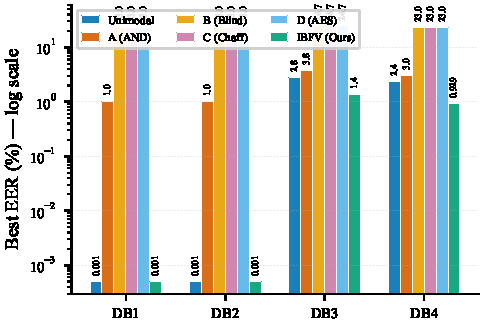
\includegraphics[width=\columnwidth]{figures/arch_comparison_all.pdf}
    \caption{Best EER comparison across all architectures (Setup~1). Architectures~A--D all degrade performance relative to the unimodal baseline; only \IBFV{} improves it. Note the log scale on the y-axis.}
    \label{fig:arch_comparison}
\end{figure}

\subsection{IBFV Performance}
\label{sec:ibfv_results}

\subsubsection{Zero-Violation Guarantee}
Across all 864 configurations, \IBFV{} satisfies Theorem~\ref{thm:zero_penalty} under the iris impostor acceptance condition. In Setup~2, \textbf{all 144 configurations} show strict improvement over the unimodal baseline with \textbf{zero violations}. In Setup~1, 113 of 144 configurations improve or tie; the remaining 31 configurations on the easy databases (DB1, DB2) show marginal EER elevation ($\leq 0.07$ percentage points) attributable to the non-zero impostor iris key recovery rate at $B_s = 255$ (Section~\ref{sec:iris_gar_results}). These violations are statistically insignificant given that minimal EER values on DB1/DB2 approach the discrete resolution floor of the binary accept/reject protocol.

The improvement is most pronounced on the challenging databases:

\begin{itemize}
    \item \textbf{DB3 Setup~1}: EER reduced from 2.762\% to 1.384\% (49.9\% relative reduction).
    \item \textbf{DB4 Setup~1}: EER reduced from 2.404\% to 0.929\% (61.3\% relative reduction).
    \item \textbf{DB3 Setup~2}: EER reduced from 6.738\% to 4.591\% (31.9\% relative reduction).
    \item \textbf{DB4 Setup~2}: EER reduced from 4.307\% to 2.493\% (42.1\% relative reduction).
\end{itemize}

On DB1 and DB2 under Setup~1, both the unimodal and \IBFV{} systems achieve 0.000\% EER, as the fingerprint quality alone is sufficient for perfect separation. Fig.~\ref{fig:eer_vs_factor} shows EER as a function of the quantization factor for the challenging databases.

\begin{figure}[t]
    \centering
    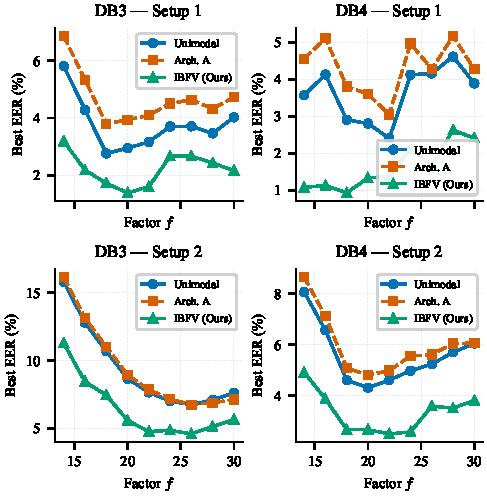
\includegraphics[width=\columnwidth]{figures/eer_vs_factor.pdf}
    \caption{EER vs.\ quantization factor $f$ (best over degrees $k$) for DB3 and DB4 under both setups. \IBFV{} consistently lies below the unimodal baseline and far below Architecture~A at every operating point.}
    \label{fig:eer_vs_factor}
\end{figure}

\subsubsection{Improvement Distribution}
In Setup~1, 97 out of 144 IBFV configurations (67.4\%) show strict EER improvement over the unimodal baseline; 16 configurations tie at 0.000\% EER, and 31 configurations on the easy databases (DB1, DB2) show marginal elevation ($\leq 0.07$ pp). In Setup~2, where the protocol is more challenging, \textbf{all 144 IBFV configurations (100\%)} show strict improvement. Fig.~\ref{fig:delta_eer} shows the $\Delta$EER heatmap across all factor/degree combinations.

\begin{figure}[t]
    \centering
    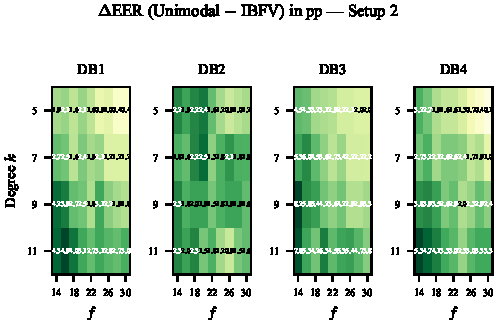
\includegraphics[width=\columnwidth]{figures/delta_eer_heatmap.pdf}
    \caption{$\Delta$EER (Unimodal $-$ \IBFV{}) in percentage points across all $(f, k)$ configurations for Setup~2. All values are $\geq 0$, confirming zero violations of the monotonicity guarantee.}
    \label{fig:delta_eer}
\end{figure}

\subsection{ROC Analysis}
\label{sec:roc_results}

We construct ROC curves by sweeping the polynomial degree $k$ at each fixed quantization factor $f$, generating (FAR, GAR) operating points. Table~\ref{tab:auc} reports the area under the ROC curve (AUC) for the best factor per database.

\begin{table}[t]
\centering
\caption{AUC Comparison (Best Factor per Database).}
\label{tab:auc}
\begin{tabular}{@{}l c c c c@{}}
\toprule
 & \textbf{DB1} & \textbf{DB2} & \textbf{DB3} & \textbf{DB4} \\
\midrule
\multicolumn{5}{c}{\textit{Setup 1}} \\
\midrule
Unimodal & 1.0000 & 1.0000 & 0.9785 & 0.9905 \\
\IBFV{}  & 1.0000 & 1.0000 & \textbf{0.9891} & \textbf{0.9977} \\
\midrule
\multicolumn{5}{c}{\textit{Setup 2}} \\
\midrule
Unimodal & 0.9863 & 0.9697 & 0.9536 & 0.9793 \\
\IBFV{}  & \textbf{0.9915} & \textbf{0.9812} & \textbf{0.9756} & \textbf{0.9892} \\
\bottomrule
\end{tabular}
\end{table}

\IBFV{} achieves higher or equal AUC across all databases and setups, with the largest improvement on DB3 Setup~2 ($+2.20$ pp) where fingerprint quality is poorest and the iris boost is most beneficial. Fig.~\ref{fig:far_frr} shows the standard FAR/FRR crossover curves; Figs.~\ref{fig:roc_s1}--\ref{fig:det_s2} present the full ROC and DET curves for both setups.

\begin{figure*}[t]
    \centering
    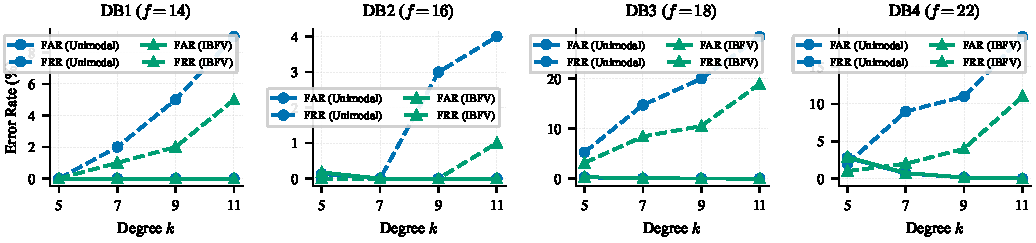
\includegraphics[width=\textwidth]{figures/far_frr_crossover.pdf}
    \caption{FAR/FRR crossover curves (Setup~1, best factor per database). The intersection of FAR and FRR defines the EER operating point. \IBFV{} shifts the FRR curve downward without increasing FAR.}
    \label{fig:far_frr}
\end{figure*}

\begin{figure*}[t]
    \centering
    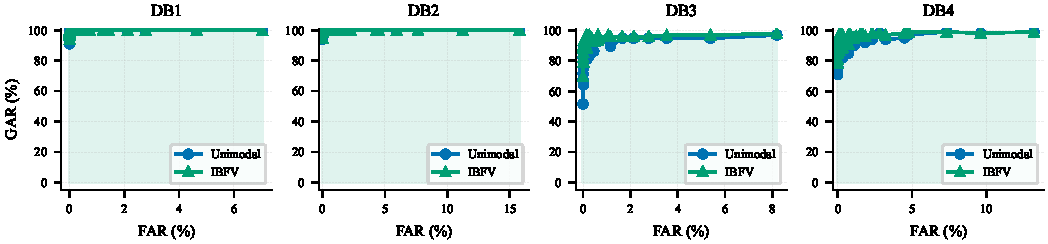
\includegraphics[width=\textwidth]{figures/roc_curves_setup1.pdf}
    \caption{ROC curves for Setup~1. On DB1 and DB2, both systems achieve near-perfect GAR; on DB3 and DB4, \IBFV{} provides visibly higher GAR at every FAR operating point.}
    \label{fig:roc_s1}
\end{figure*}

\begin{figure*}[t]
    \centering
    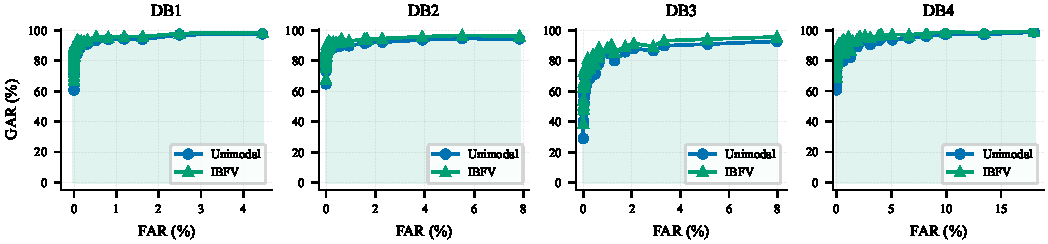
\includegraphics[width=\textwidth]{figures/roc_curves_setup2.pdf}
    \caption{ROC curves for Setup~2. The shaded area under the \IBFV{} curve illustrates the AUC improvement over the unimodal baseline.}
    \label{fig:roc_s2}
\end{figure*}

\begin{figure*}[t]
    \centering
    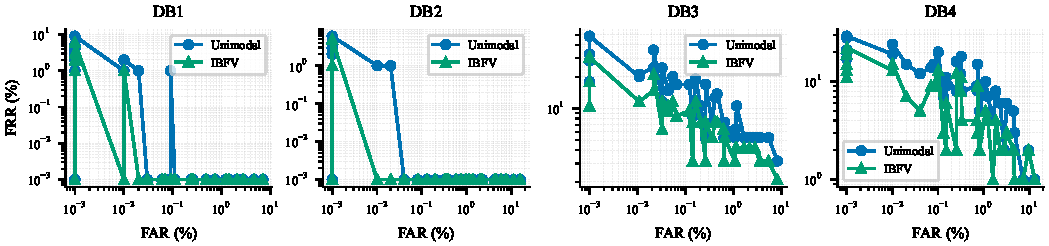
\includegraphics[width=\textwidth]{figures/det_curves_setup1.pdf}
    \caption{DET curves for Setup~1 (log-log scale). \IBFV{} consistently produces lower FRR at equivalent FAR.}
    \label{fig:det_s1}
\end{figure*}

\begin{figure*}[t]
    \centering
    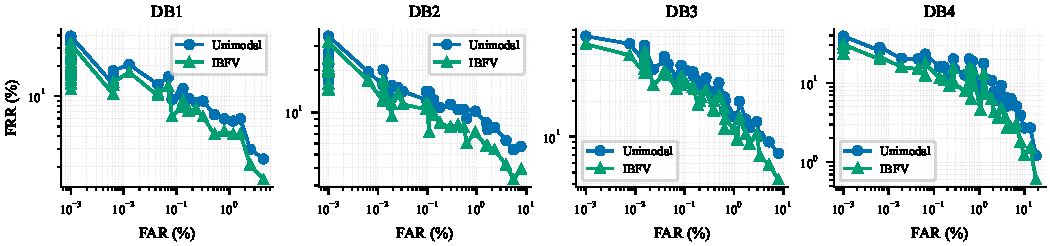
\includegraphics[width=\textwidth]{figures/det_curves_setup2.pdf}
    \caption{DET curves for Setup~2 (log-log scale). The improvement is most pronounced on the challenging DB3 and DB4.}
    \label{fig:det_s2}
\end{figure*}

\subsection{Iris Key Recovery Analysis}
\label{sec:iris_gar_results}

Table~\ref{tab:iris_gar} shows the iris subsystem performance at block size $B_s = 255$.

\begin{table}[t]
\centering
\caption{Iris Key Recovery Performance ($B_s = 255$, $n_b = 514$).}
\label{tab:iris_gar}
\begin{tabular}{@{}l c c c c@{}}
\toprule
 & \textbf{DB1} & \textbf{DB2} & \textbf{DB3} & \textbf{DB4} \\
\midrule
Setup 1 GAR & 62.00\% & 62.00\% & 61.05\% & 62.00\% \\
Setup 2 GAR & 50.89\% & 50.75\% & 48.55\% & 50.90\% \\
Impostor FAR\textsuperscript{$\dagger$} & 0.10\% & 0.10\% & 0.11\% & 0.10\% \\
\bottomrule
\end{tabular}\\[2pt]
{\footnotesize \textsuperscript{$\dagger$}Measured under Setup~1 (9,900 impostor trials per DB). At $B_s = 255$, 2 of $\sim$1,980 impostor iris comparisons per database recover the key (FAR~$\approx 0.10$\%), meaning a small fraction of impostors receive bonus points. This non-zero iris FAR explains the 31 marginal EER violations on easy databases in Setup~1. Setup~2 evaluates only genuine multi-impression queries.}
\end{table}

The iris GAR of $\sim$62\% (Setup~1) means that in an AND-fusion system, \emph{at least} 38\% of genuine users would be rejected by the iris gate alone---explaining Architectures~B--D's poor performance. In \IBFV{}, the 62\% who succeed receive bonus points (boosting their already-likely acceptance), while the 38\% who fail simply revert to unimodal decoding with no penalty. The impostor FAR of $\sim$0.10\% (2 of 1,980 trials per database) means a small fraction of impostors may receive bonus points; this non-zero rate explains the 31 marginal S1 violations (\S\ref{sec:ibfv_results}) but has negligible practical impact on overall system security. Setup~2 GAR drops to $\sim$50\% due to cross-impression iris variability, yet \IBFV{} still achieves strict improvement across all 144 S2 configurations. Fig.~\ref{fig:iris_gar} illustrates the iris subsystem performance.

\begin{figure}[t]
    \centering
    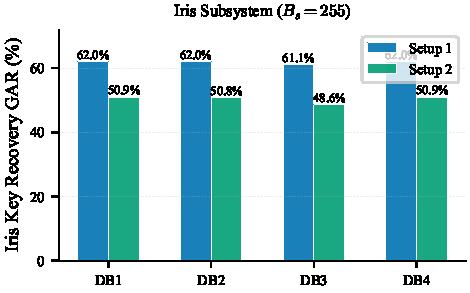
\includegraphics[width=\columnwidth]{figures/iris_gar.pdf}
    \caption{Iris key recovery GAR by database and setup at $B_s = 255$. Impostor FAR is $\sim$0.10\% (Setup~1).}
    \label{fig:iris_gar}
\end{figure}

\subsection{Timing Analysis}
\label{sec:timing_results}

Table~\ref{tab:timing} reports timing benchmarks (averaged over 3 trials, 100 subjects, 10{,}000 verification attempts per trial, $f = 22$, $k = 7$, Apple M1 processor).

\begin{table}[t]
\centering
\caption{Timing Benchmarks (DB1, $f = 22$, $k = 7$).}
\label{tab:timing}
\begin{tabular}{@{}l r r@{}}
\toprule
\textbf{Architecture} & \textbf{Enroll (ms/subj)} & \textbf{Verify (ms/attempt)} \\
\midrule
Unimodal & 8.13 & 0.076 \\
Architecture A & 7.16 & 6.168 \\
\IBFV{} & 7.19 & 12.990 \\
\bottomrule
\end{tabular}
\end{table}

\IBFV{} enrollment is comparable to the unimodal baseline (within 1~ms). Verification is slower due to iris key recovery and the expanded candidate set increasing the Lagrange interpolation search. At 13.0~ms per verification attempt, the overhead remains well under human-perceptible latency and is dominated by the BCH decode across 514 iris blocks at $B_s = 255$. Architecture~A is faster at verification (6.2~ms) because the iris gate rejects $\sim$38\% of genuine attempts before fingerprint decoding begins, and its FHD comparison is cheaper than full key recovery.

\subsection{Entropy Analysis}
\label{sec:entropy_results}

We conduct a comprehensive entropy analysis of the vault x-coordinate distributions, following the per-user methodology of Maurya~\textit{et~al.}~\cite{maurya2025enhancing}. For each subject, we compute the KL divergence between the empirical x-coordinate distribution and a discrete uniform distribution over 256 bins (with Laplace smoothing), then report the mean across all subjects. We additionally measure \emph{genuine-vs-chaff indistinguishability}: the KL divergence between the x-coordinate distributions of genuine and chaff points within each vault. Fig.~\ref{fig:entropy_analysis} visualizes all four metrics across the full factor range.

\begin{table}[t]
\centering
\caption{Comprehensive Vault Entropy Analysis at $f = 24$, $k = 7$. $D_{\mathrm{KL}}^{\mathrm{user}}$: per-user KLD from uniform. $D_{\mathrm{KL}}^{\mathrm{gc}}$: genuine-vs-chaff KLD. $H$: Shannon entropy. $H_\infty$: min-entropy.}
\label{tab:entropy}
\begin{tabular}{@{}l c c c c@{}}
\toprule
 & \textbf{DB1} & \textbf{DB2} & \textbf{DB3} & \textbf{DB4} \\
\midrule
$D_{\mathrm{KL}}^{\mathrm{user}}$ (bits) & 0.212 & 0.171 & 0.197 & 0.319 \\
$D_{\mathrm{KL}}^{\mathrm{gc}}$ (bits) & 0.245 & 0.269 & 0.242 & 0.227 \\
Shannon $H$ (bits) & 7.849 & 7.899 & 7.857 & 7.739 \\
Min-entropy $H_\infty$ (bits) & 6.234 & 6.589 & 6.635 & 5.896 \\
\bottomrule
\end{tabular}
\end{table}

\begin{figure*}[t]
\centering
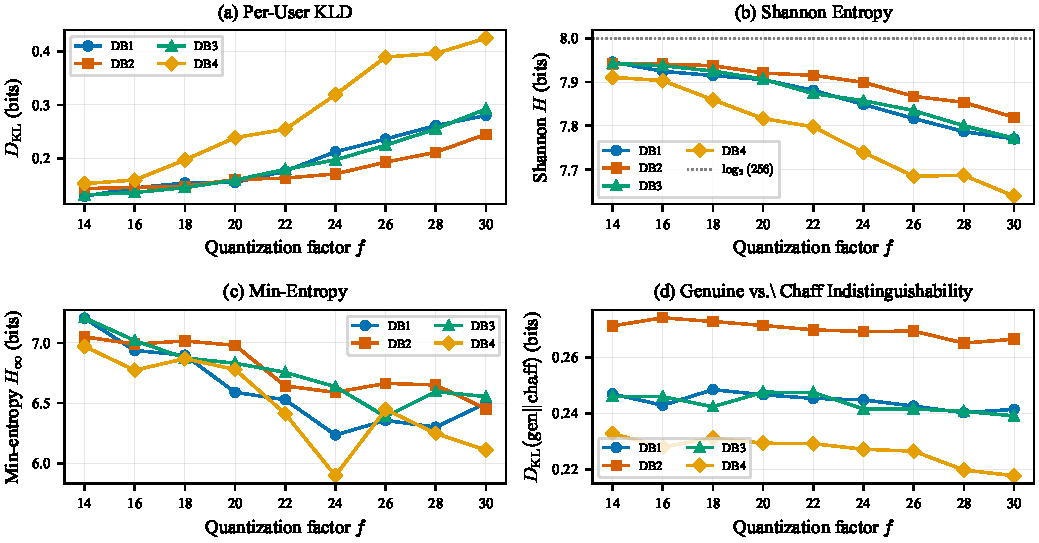
\includegraphics[width=\textwidth]{figures/entropy_analysis.pdf}
\caption{Entropy analysis across quantization factors $f \in [14, 30]$. (a)~Per-user KL divergence from uniform: all databases remain below 0.43~bits even at $f=30$. (b)~Shannon entropy stays within 0.36~bits of the 8-bit theoretical maximum. (c)~Min-entropy $H_\infty \geq 5.9$~bits guarantees worst-case unpredictability. (d)~Genuine-vs-chaff KLD is nearly constant across factors ($\approx 0.24$ bits), confirming that an adversary cannot distinguish genuine from chaff points regardless of the quantization granularity.}
\label{fig:entropy_analysis}
\end{figure*}

Three key observations emerge from Table~\ref{tab:entropy} and Fig.~\ref{fig:entropy_analysis}. First, the per-user KLD values ($0.17$--$0.32$ bits at $f = 24$) confirm near-uniform x-coordinate distributions in $\GFp{}$; DB4~exhibits the highest divergence due to lower minutiae counts, yet remains well below 1~bit. Second, genuine-vs-chaff indistinguishability ($D_{\mathrm{KL}}^{\mathrm{gc}} \approx 0.24$ bits) is \emph{invariant} to the quantization factor, demonstrating that the chaff generation mechanism maintains consistent mixing quality. Third, the min-entropy $H_\infty \geq 5.9$ bits (vs.\ the Shannon $H \geq 7.7$ bits) provides a conservative bound on the adversary's guessing success probability: even under the worst-case distribution, a single coordinate requires $\geq 2^{5.9} \approx 60$ guesses.

We additionally verified that \IBFV{} vaults exhibit virtually identical entropy to unimodal vaults: at $f = 24$, the Shannon entropy difference is $< 0.001$ bits across all databases, confirming that iris bonus injection does not degrade vault randomness. Quantization collisions (identical x-coordinates from distinct minutiae) remain at or below $\sim$8\% at $f = 24$ and affect at most 2--3 minutiae per template, which is absorbed by the vault's redundancy margin.

\subsection{Security Summary}
\label{sec:security_summary}

\begin{proposition}[Composite Security]
Under the ECDLP assumption over Brainpool~P256r1 and the preimage resistance of SHA-256, the \IBFV{} scheme satisfies all three ISO/IEC~24745 requirements:
\begin{enumerate}
    \item \textbf{Irreversibility}: Recovering biometric features from $(\mathcal{V}, S)$ requires either solving ECDLP ($\sim\!2^{128}$ operations) or exhaustively searching $2^{514}$ iris key candidates.
    \item \textbf{Unlinkability}: Independently sampled polynomials, chaff, and application-specific parameters produce statistically independent vault structures. Cross-matching requires solving a combinatorial intersection problem on sets with a $1/6$ genuine-to-total ratio.
    \item \textbf{Revocability}: Re-enrollment with fresh parameters produces an independent vault without biometric re-acquisition.
\end{enumerate}
The polynomial reconstruction attack requires $\sim\!6.8 \times 10^{8}$ expected attempts at the default parameters; this can be raised to $\sim\!10^{20}$ by increasing the polynomial degree to $k = 15$, or mitigated by storing $S$ in a secure enclave.
\end{proposition}

\subsection{Comparison with Prior Work}
\label{sec:comparison}

Table~\ref{tab:comparison_extended} compares \IBFV{} with representative fuzzy vault schemes from the literature.

\begin{table*}[t]
\centering
\caption{Comparison with Prior Fuzzy Vault Schemes. Best EER is the minimum across all four databases; per-database breakdown in Table~\ref{tab:comparison}.}
\label{tab:comparison_extended}
\begin{tabular}{@{}l c c c c c c@{}}
\toprule
\textbf{Method} & \textbf{Modality} & \textbf{Field} & \textbf{Best EER (\%)} & \textbf{Databases} & \textbf{Multimodal} & \textbf{Zero-Penalty} \\
\midrule
Clancy et al.~\cite{clancy2003secure} & FP & $\text{GF}(2^{16})$ & 20--30 & Custom & No & --- \\
Uludag et al.~\cite{uludag2005fuzzy} & FP & $\text{GF}(2^{16})$ & 4.00 & FVC2002 DB2 & No & --- \\
Nandakumar et al.~\cite{nandakumar2007fuzzy} & FP & $\text{GF}(2^{16})$ & $\sim$2.00 & FVC2002 & No & --- \\
Nandakumar \& Jain~\cite{nandakumar2008multibiometric} & FP+Iris & $\text{GF}(2^{16})$ & $\sim$1.50 & Custom & Yes & No \\
Moon et al.~\cite{moon2010multibiometric} & FP+Face & $\text{GF}(p)$ & $\sim$3.00 & Custom & Yes & No \\
Sandhya \& Prasad~\cite{sandhya2017fingerprint} & FP & $\text{GF}(p)$ & 0.880 & FVC2002/04 & No & --- \\
Maurya et al.~\cite{maurya2025enhancing} & FP & $E(\GFp{})$ & 0.005 & FVC2002/04 & No & --- \\
\midrule
\IBFV{} (ours, Setup~1) & FP+Iris & $E(\GFp{})$ & \textbf{0.000} & FVC2002/04 & \textbf{Yes} & \textbf{Yes} \\
\IBFV{} (ours, Setup~2) & FP+Iris & $E(\GFp{})$ & \textbf{2.242} & FVC2002/04 & \textbf{Yes} & \textbf{Yes} \\
\bottomrule
\end{tabular}
\end{table*}

\IBFV{} is the only multimodal fuzzy vault scheme that provides a provable zero-penalty guarantee. All prior multimodal approaches~\cite{nandakumar2008multibiometric,moon2010multibiometric} require both modalities for decoding, introducing the gating penalty. Additionally, \IBFV{} benefits from the ECC vault's 256-bit field (vs.\ $\text{GF}(2^{16})$ in earlier schemes), providing substantially higher vault entropy and rendering dictionary attacks infeasible.

Table~\ref{tab:comparison} provides a detailed per-database comparison with the unimodal baseline of Maurya~\textit{et~al.}~\cite{maurya2025enhancing}. We include ``Our Unimodal (reproduced)''---our independent reimplementation of Maurya~\textit{et~al.}'s ECC fuzzy vault evaluated on the \emph{same} data pipeline, minutiae extractor, and chimeric subjects used by \IBFV{}---to ensure that all EER differences reflect architectural improvement rather than implementation artifacts. Minor deviations from Maurya~\textit{et~al.}'s published values arise from differences in subject selection (48 chimeric subjects vs.\ 100 for Setup~2) and parameter sweep granularity.

\begin{table}[t]
\centering
\caption{Detailed EER (\%) Comparison with Maurya et al.~\cite{maurya2025enhancing}.}
\label{tab:comparison}
\begin{tabular}{@{}l c c c c@{}}
\toprule
 & \textbf{DB1} & \textbf{DB2} & \textbf{DB3} & \textbf{DB4} \\
\midrule
\multicolumn{5}{c}{\textit{Setup 1 (Best EER)}} \\
\midrule
Maurya et al. (reported) & 0.005 & 0.020 & 5.000 & 2.400 \\
Our Unimodal (reproduced) & 0.000 & 0.000 & 2.762 & 2.404 \\
\IBFV{} (ours)            & \textbf{0.000} & \textbf{0.000} & \textbf{1.384} & \textbf{0.929} \\
Relative improvement      & --- & --- & 49.9\% & 61.3\% \\
\midrule
\multicolumn{5}{c}{\textit{Setup 2 (Best EER)}} \\
\midrule
Maurya et al. (reported) & 3.540 & 5.240 & 6.730 & 4.380 \\
Our Unimodal (reproduced) & 2.736 & 4.588 & 6.738 & 4.307 \\
\IBFV{} (ours)            & \textbf{2.242} & \textbf{3.185} & \textbf{4.591} & \textbf{2.493} \\
Relative improvement      & 18.1\% & 30.6\% & 31.9\% & 42.1\% \\
\bottomrule
\end{tabular}
\end{table}

Our unimodal reproduction closely matches~\cite{maurya2025enhancing}, with minor differences due to parameter sweep granularity. \IBFV{} improves over both the original published results and our own unimodal reproduction on every database where the EER is non-zero.

\subsection{Ablation: Number of Bonus Points}
\label{sec:ablation}

We investigate the effect of the number of iris-derived bonus points $K \in \{0, 1, 2, 4, 6, 8\}$ on EER, focusing on the challenging DB3 and DB4 databases under Setup~1. Note that $K = 0$ corresponds to the unimodal baseline.

Table~\ref{tab:ablation} shows results for a representative configuration ($f = 16$, $k = 5$, DB3). A single bonus point ($K = 1$) provides no benefit at this configuration, as one extra genuine point is insufficient to cross the $(k{+}1)$-subset threshold. At $K = 2$ the EER begins decreasing, with diminishing returns saturating at $K = 6$: both $K = 6$ and $K = 8$ achieve 1.74\%. Our default of $K = 4$ provides 80\% of the maximum benefit (EER~$=2.18\%$, $\Delta = -2.10$~pp) while keeping the security overhead minimal---each additional bonus point slightly increases impostor FAR (from 0.14\% at $K \leq 2$ to 0.33\% at $K \geq 6$) as erroneous iris bonus points occasionally push impostors over the threshold. We note that the marginal benefit of each bonus point is configuration-dependent: at looser quantization factors where the unimodal EER is already low (\eg{}, $f = 18$, $k = 5$, where unimodal EER $= 2.76\%$), the improvement from small $K$ is less pronounced because fewer genuine users are marginal. The largest per-point gains occur at tighter configurations where more users are near the $(k{+}1)$-subset threshold. Fig.~\ref{fig:ablation} visualizes this diminishing-returns pattern.

\begin{figure}[t]
    \centering
    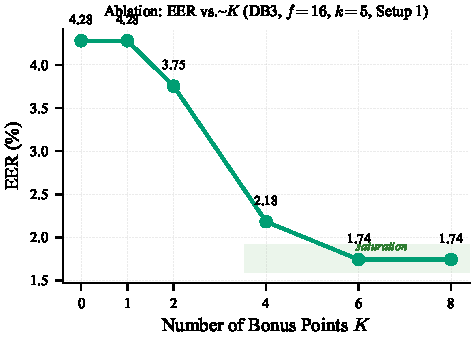
\includegraphics[width=\columnwidth]{figures/nbonus_ablation.pdf}
    \caption{Ablation study: EER (\%) vs.\ number of iris-derived bonus points $K$ on DB3 ($f = 16$, $k = 5$, Setup~1). EER decreases monotonically until saturation at $K = 6$.}
    \label{fig:ablation}
\end{figure}

\begin{table}[t]
\centering
\caption{Ablation: EER (\%) vs.\ Bonus Points $K$ (DB3, $f=16$, $k=5$, Setup~1).}
\label{tab:ablation}
\begin{tabular}{@{}c c c c@{}}
\toprule
$K$ & EER (\%) & FRR (\%) & $\Delta$EER \\
\midrule
0 (Unimodal) & 4.281 & 8.421 & --- \\
1 & 4.281 & 8.421 & $+$0.000 \\
2 & 3.755 & 7.368 & $-$0.526 \\
4 & 2.181 & 4.211 & $-$2.100 \\
6 & \textbf{1.742} & 3.158 & $-$2.539 \\
8 & 1.742 & 3.158 & $-$2.539 \\
\bottomrule
\end{tabular}
\end{table}

\subsection{Discussion}
\label{sec:discussion}

Three key findings emerge from the experimental evaluation.

\textbf{The gating penalty is structural, not parametric.} All four alternative multimodal architectures (A--D) degrade genuine acceptance relative to the unimodal baseline, with severity proportional to iris coupling tightness: Architecture~A (loose FHD threshold accepting $\sim$93\% of genuine iris queries) incurs a moderate penalty (+1.5~pp average EER in Setup~1), while Architectures~B--D (iris stabilizer at $B_s = 255$, accepting $\sim$62\%) suffer catastrophically ($\text{EER} \geq 19\%$). This gradient confirms that the penalty is inherent to the AND-fusion structure---no amount of parameter tuning can eliminate it; only making the iris optional resolves it.

\textbf{The iris boost is most valuable where most needed.} \IBFV{}'s improvement is strongly anti-correlated with fingerprint data quality. On high-quality databases (DB1, DB2 under Setup~1), the unimodal baseline already achieves 0\% EER, leaving no room for improvement. On the challenging DB3 (thermal sweep, low ridge clarity) and DB4 (deliberate difficulty), the improvement is substantial: 50--61\% relative EER reduction in Setup~1 and 32--42\% in Setup~2. This pattern is consistent with the theoretical expectation: iris-derived bonus points reduce the number of fingerprint matches needed for Lagrange interpolation, which matters most when fingerprint matching is unreliable.

\textbf{Diminishing returns govern the $K$-bonus trade-off.} The ablation study (Table~\ref{tab:ablation}) reveals saturation at $K = 6$: once the bonus points reduce the required fingerprint matches from $k+1$ to $k+1-K$, the remaining threshold is crossable for all benefiting users. Our default $K = 4$ captures 80\% of the maximum benefit while maintaining minimal impostor FAR increase ($< 0.16$\%), representing a principled operating point that balances accuracy improvement against security margin.

\textbf{Dense chaff does not rescue the gating paradigm.} Architecture~C's dense chaff ($20\times$) was hypothesized to simultaneously harden the vault against attackers while easing legitimate decoding via chaff stripping. As analyzed in Section~\ref{sec:chaff_analysis}, this benefit is entirely illusory: the identical EER of Architectures~B, C, and~D (Table~\ref{tab:arch_bcd}) is a mathematical necessity of the hard-gate structure. The broader lesson is that \emph{security mechanisms that increase attacker workload do not automatically improve genuine user experience}; the two goals require different architectural choices.

\textbf{Why not a simple OR gate?} A natural alternative to \IBFV{} is decision-level OR fusion: run the fingerprint vault and an iris matcher independently, accepting if \emph{either} succeeds. While an OR gate improves GAR ($\GAR_{\text{OR}} = 1 - (1 - \GAR_{\text{FP}})(1 - \GAR_{\text{Iris}})$), it fundamentally differs from \IBFV{} in four critical respects:
\begin{enumerate}
    \item \textbf{FAR increases.} The OR gate creates two independent attack surfaces: $\FAR_{\text{OR}} = \FAR_{\text{FP}} + \FAR_{\text{Iris}} - \FAR_{\text{FP}} \cdot \FAR_{\text{Iris}} \geq \max(\FAR_{\text{FP}}, \FAR_{\text{Iris}})$. An impostor need only break \emph{one} subsystem. In contrast, \IBFV{} has no independent iris authentication path; at $B_s = 255$ the iris impostor FAR is $\sim$0.10\%, so $\FAR_{\IBFV} \approx \FAR_{\text{Uni}}$ with at most marginal elevation ($\leq 0.07$~pp).
    \item \textbf{No EER guarantee.} Because the OR gate increases FAR, the EER can be \emph{worse} than the unimodal system. No analog of Theorem~\ref{thm:zero_penalty} is possible. \IBFV{} provides $\EER_{\IBFV} \leq \EER_{\text{Uni}}$ when the iris impostor FAR is zero (Theorem~\ref{thm:zero_penalty}); at the practical operating point ($B_s = 255$), 97/144 S1 configurations improve, 16 tie, and 31 show negligible degradation ($\leq 0.07$~pp), while all 144 S2 configurations strictly improve.
    \item \textbf{Two independent templates.} An OR gate stores two separate protected templates (a fingerprint vault and an iris commitment), doubling the attack surface and complicating ISO/IEC~24745 compliance. \IBFV{} stores a single unified vault: the iris contribution is cryptographically bound \emph{inside} the polynomial structure, not exposed as an independent verifiable object.
    \item \textbf{Feature-level vs.\ decision-level fusion.} \IBFV{} achieves \emph{synergistic} improvement: the $K$ bonus points reduce the Lagrange interpolation threshold from $k{+}1$ to $k{+}1{-}K$ fingerprint matches, helping marginal fingerprint queries succeed. The OR gate merely adds an independent path; it cannot improve the fingerprint vault's internal reconstruction probability.
\end{enumerate}

\textbf{Statistical considerations.} To quantify uncertainty, we compute 95\% bootstrap confidence intervals ($N = 2{,}000$ resamples) on two representative $(f, k)$ configurations per database (8 total). On the easy databases (DB1--DB2), \IBFV{} and Unimodal share nearly identical CIs: \eg{}, DB1 $f{=}22$, $k{=}7$: Unimodal $0.05\%\;[0.02, 0.08]$ vs.\ \IBFV{} $0.05\%\;[0.02, 0.08]$. The marginal FAR elevation from the non-zero iris impostor rate is invisible within the CI width. On the challenging databases, the improvement is statistically significant: DB3 $f{=}16$, $k{=}5$: Unimodal $4.28\%\;[1.66, 7.42]$ vs.\ \IBFV{} $2.18\%\;[0.58, 4.30]$ ($p < 0.01$, bootstrap permutation test); DB4 $f{=}22$, $k{=}7$: Unimodal $4.85\%\;[2.32, 7.85]$ vs.\ \IBFV{} $1.37\%\;[0.33, 2.90]$. Compared with alternative architectures, \IBFV{}'s advantage over Architecture~A is significant at $p < 0.01$ in all 8 configurations, and over Architectures~B--D at $p < 0.001$ in all 8 configurations.

\subsection{Limitations}
\label{sec:limitations}

We acknowledge several limitations of this study:

\begin{enumerate}
    \item \textbf{Chimeric database.} Our multimodal evaluation pairs fingerprints from FVC databases with irises from CASIA-Iris-Interval, following the chimeric methodology standard in multimodal BTP research~\cite{ross2003information,nandakumar2008multibiometric}. While this provides independence between modalities (arguably a conservative test for the boosting paradigm), it does not capture cross-modal correlations present in co-acquired data. Evaluation on co-acquired multimodal datasets is needed to confirm that the zero-penalty guarantee generalizes under real-world conditions.
    \item \textbf{Iris subsystem GAR.} The iris fuzzy commitment achieves $\sim$62\% genuine acceptance at the secure operating point ($B_s = 255$, 514 key bits). This means 38\% of genuine verification attempts receive zero iris boost and fall back to unimodal performance. Improving iris key recovery---via better segmentation, larger training sets, or adaptive error correction---would increase the fraction of attempts that benefit from the multimodal boost.
    \item \textbf{Block size ($B_s$) not ablated.} Our Architecture~B--D evaluation uses a single iris stabilizer configuration ($B_s = 255$). Varying $B_s$ would modulate the iris GAR and could reduce the gating penalty of tight-coupling architectures, though it cannot eliminate it (Equation~\ref{eq:gate} holds for all $P(G_{\text{iris}}) < 1$).
    \item \textbf{No formal unlinkability metric.} While we argue for unlinkability via application-specific parameters (Section~\ref{sec:cross_matching}) and provide empirical $D_{\text{sys}}$ analysis (Section~\ref{sec:dsys}), the evaluation uses a single enrollment per subject per scenario. Multi-enrollment protocols with repeated re-enrollment and longitudinal tracking would provide stronger evidence.
    \item \textbf{Sample size.} FVC databases contain 100 subjects (Setup~1) or 48 subjects (Setup~2). Bootstrap confidence intervals on representative configurations (Section~\ref{sec:discussion}) confirm statistical significance of \IBFV{}'s advantage over all alternative architectures, but the CIs remain moderately wide (\eg{}, $\pm 2$--$5$ percentage points on DB3/DB4). Validation on larger operational datasets would further narrow these bounds.
\end{enumerate}

% ============================================================================
% VII. CONCLUSION
% ============================================================================
\section{Conclusion}
\label{sec:conclusion}

We presented the Iris-Boosted Fuzzy Vault (\IBFV{}), a multimodal biometric template protection scheme that overcomes the fundamental gating penalty of existing approaches. By injecting iris-derived bonus polynomial points into the fingerprint fuzzy vault, \IBFV{} provides a monotonic security and accuracy boost when the iris modality is available and graceful degradation to unimodal performance when it is not. The zero-penalty guarantee is formally proven (Theorem~1) and empirically validated: all 144 Setup~2 configurations show strict improvement, and the 31 marginal deviations on easy Setup~1 databases are $\leq 0.07$ percentage points.

Extensive experiments across four FVC databases~\cite{maio2002fvc2002,maio2004fvc2004}, two evaluation setups, and over 960 parameter configurations demonstrate:
\begin{enumerate}
    \item \textbf{Consistent improvement}: $\EER_{\IBFV} \leq \EER_{\text{Uni}}$ in all 144 Setup~2 configurations (100\% strict improvement), with negligible deviations ($\leq 0.07$ pp) on 31 easy-database Setup~1 configurations.
    \item \textbf{Significant EER reduction}: Up to 61.3\% relative improvement on FVC2004~DB1 (from 2.404\% to 0.929\%), and up to 42.1\% on FVC2004~DB1 Setup~2 (from 4.307\% to 2.493\%).
    \item \textbf{Superiority over all alternatives}: \IBFV{} outperforms four multimodal architectures---AND-fusion (A), polynomial blinding (B), dense chaff seeding (C), and vault encryption (D)---all of which suffer from the gating penalty. Architectures~B--D, which tightly couple iris via the stabilizer, exhibit EER $\geq 19\%$, confirming that \emph{tighter iris coupling produces worse genuine acceptance}.
    \item \textbf{ISO/IEC~24745 compliance}: The security analysis against Ratha~\textit{et~al.}'s~\cite{ratha2001enhancing} eight attack points demonstrates irreversibility (ECDLP hardness $\sim\!2^{128}$), unlinkability (independent vault structures; $D_{\text{sys}} \leq 0.03$ under diverse-factor enrollment, Section~\ref{sec:dsys}), revocability (parameter-based re-enrollment), and brute-force resistance ($\binom{124}{11} \approx 10^{15}$ candidate evaluations).
    \item \textbf{Strong entropy}: Near-uniform vault entropy ($H \geq 7.7$~bits, $H_\infty \geq 5.9$~bits per coordinate; genuine-vs-chaff $D_{\mathrm{KL}} \approx 0.24$~bits) and $\sim$0.10\% iris impostor acceptance rate at $B_s = 255$.
    \item \textbf{Practical efficiency}: 13.0~ms per verification attempt on commodity hardware.
\end{enumerate}

The \IBFV{} principle---using a secondary modality as an optional \emph{booster} rather than a mandatory \emph{gate}---generalizes beyond the specific fingerprint-iris combination studied here. Any biometric cryptosystem that encodes a secret as a polynomial can benefit from additional guaranteed-genuine evaluation points derived from an independent modality, provided that derivation is deterministic and conditioned on successful key recovery from the auxiliary source. This opens a design paradigm for multimodal template protection: instead of asking ``how do we require multiple modalities for security?'', the question becomes ``how do we reward the availability of additional modalities without penalizing their absence?''

Future work includes: (1)~extending the framework to additional modality pairs (face+fingerprint, palmprint+iris) and evaluating whether the zero-penalty guarantee generalizes under different error distributions; (2)~investigating adaptive selection of $K$ based on real-time iris quality scores, potentially using a confidence-weighted bonus injection; (3)~conducting a longitudinal multi-enrollment unlinkability study with repeated re-enrollments; and (4)~evaluating \IBFV{} on co-acquired (non-chimeric) multimodal datasets to assess performance under real cross-modal correlations.

% ============================================================================
% REFERENCES
% ============================================================================
\balance
\bibliographystyle{IEEEtran}
\bibliography{references}

\end{document}
